% \chapter{Diseño de los sistemas ópticos}         % o \chapter{Resultados y Discusión}

% En este capítulo se describe el proceso que se lleva a cabo para la determinación de los componentes ópticos necesarios para cumplir los requerimientos ópticos de la misión C3. En un primer momento, se describen los criterios a tener en cuenta para el diseño de la HuMath\textregistered QBee, en los cuales se describen los parámetros mecánicos, ópticos y enegéticos que debe cumplir el dispositivo HuMath \textregistered QBee para operar en las condiciones estimadas. Luego, se describe el proceso iterativo de diseño óptico, en el cual se describen los candidatos de objetivos y sensores ópticos tenidos en cuenta. De estos elementos, se obtienen caraterísticas de resolución y campo de visión teóricos a partir con el fin de tener un criterio de selección y escoger una configuración óptima entre los candidatos.

% %===============================================================
% \section{Diseño del sistema multiespectral \textit{HuMath \textregistered QBee}}
% %===============================================================

% La ruta de desarrollo de la HuMath \textregistered QBee partió de una matriz de ocho sistemas   candidatos; de ellos se seleccionaron las dos configuraciones VIS + NIR que mejor satisfacen las restricciones de misión impuestas por el consorcio
% EAFIT–KTH. A continuación se describe el hilo de razonamiento que condujo al diseño final.

% %---------------------------------------------------------------
% \subsection{Requerimientos y criterios ópticos}
% %---------------------------------------------------------------

% Los criterios que guiaron la selección de cada sub‑módulo fueron:

% \begin{itemize}
%     \item \textbf{Resolución espacial} - El objetivo debe ofrecer una MTF (30\,\% de contraste) 
%           \textbf{$\geq 40\;lp/mm$}, lo que garantiza la capacidad de resolver los objetos 
%           de las dimensiones indicadas en la Tabla~\ref{tab:req_vs_obj}.
          
%     \item \textbf{Campo de visión} - El ángulo AFOV debe cubrir una extensión de suelo suficiente para realizar análisis extensivos de parcelas, bosques, cultivos, ríos, carreteras, zonas urbanas, entre otras estrucutras terrestres de interés. Por lo anterior, es ideal que el sistema tenga un campo de visión que vaya desde algunas decenas de metros hasta los kilometros, dependiendo de la altura de trabajo.
    
%     \item \textbf{Condiciones de iluminación} - La iluminación de la escena debe corresponder a iluminación ambeinte diurna.
    
%     \item \textbf{Masa y volumen} - El conjunto óptico‑electrónico debe cumplir las 
%           restricciones de carga útil de la aeronave del Proyecto C3, 
%           de modo que se mantenga un tiempo de vuelo de 3 h.  
%           En la práctica esto implica una masa total $\leq 2\;\text{kg}$ 
%           y un volumen aproximado de $100\times100\times150\;\text{mm}^{3}$.
          
%     \item \textbf{Coste} – Aunque el presupuesto final depende de los fondos del proyecto, 
%           para este trabajo se fija un \emph{límite máximo de \$1500 USD}.  
%           Con un presupuesto mayor podrían integrarse componentes de mayor rendimiento.
% \end{itemize}


% \begin{table}[h]
%   \centering
%   \caption{Especificaciones de misión y criterios de diseño del \textit{KBee}.}
%   \label{tab:req_vs_obj}
%   \begin{tabular}{|p{4cm}|c|}
%       \hline
%       \rowcolor[HTML]{EFEFEF}\textbf{Parámetro} & \textbf{Requisito} \\ \hline
%       Masa total del cargamento & $\leq 2\;\text{kg}$ \\ \hline
%       Dimensiones & $100 \times 100 \times 150\;\text{mm}^{3}$ \\ \hline
%       Tiempo máximo de misión & $\leq 3\;\text{h}$ \\ \hline
%       MTF (30\,\% de contraste) & $\geq 40\;\text{lp/mm}$ \\ \hline
%       Resolución en tierra @50\,m & $\leq 7.35\;\text{cm}$ \\ \hline
%       Resolución en tierra @1000\,m & $\leq 1.47\;\text{m}$ \\ \hline
%       Resolución en tierra @5000\,m & $\leq 7.35\;\text{m}$ \\ \hline
%   \end{tabular}
% \end{table}

% %---------------------------------------------------------------
% \subsection{Proceso iterativo de diseño}
% \label{sec:cad}
% %---------------------------------------------------------------

% La Tabla~\ref{tab:sys_tables} resume los ocho objetivos evaluados de
% forma preliminar.  Cada sistema se identifica por un número consecutivo y se
% caracteriza mediante distancia focal, relación de apertura, MTF al 30, \% de
% contraste y masa total del objetivo.\\

% \begin{table}[!h]
%     \centering
%     \caption{Comparativa de los objetivos candidatos frente a los criterios de diseño.
%              Entre paréntesis se indica el fabricante (EO = Edmund Optics).  El AFOV
%              se expresa en grados y corresponde al semidiámetro angular calculado
%              sobre el sensor empleado.}
%     \label{tab:sys_tables}
%     \begin{tabularx}{\linewidth}{|c|p{2.1cm}|C|C|C|C|C|}
%         \hline
%         \rowcolor[HTML]{EFEFEF}\textbf{System} & \textbf{Objetive} &
%         \textbf{Focal\, [mm]} &
%         \textbf{AFOV\, [°]} &
%         \textbf{Aperture} &
%         \textbf{MTF\,(30 \%)\, [lp/mm]} &
%         \textbf{Weight\, [g]} \\ \hline
        
%         1 & 16 mm f/16 ― HPr Series (EO)                & 16   & 42.2 & f/16 & 62  & 138 \\ \hline
%         2 & 50 mm f/2.8 ― HPr Series (EO)               & 50   & 10.1 & f/2.8& 180 & --  \\ \hline
%         3 & 25 mm f/1.8 ― HPr Series (EO)               & 25   & 27.8 & f/1.8& 40  & 78  \\ \hline
%         4 & 16 mm f/1.8 ― HPr Series (EO)               & 16   & 42.2 & f/1.8& 128 & 138 \\ \hline
%         5 & 4 mm f/1.8 ― Basler C125-0418-5M-P (Basler) & 4    & 109  & f/1.8& --  & --  \\ \hline
%         6 & 8 mm f/2.5 ― HEO Series (NIR, M12) (EO)     & 8    & 29.9 & f/2.5& 120 & 4   \\ \hline
%         7 & 8.5 mm f/1.3 ― Cr Series (EO)               & 8.5  & 28.2 & f/1.8& 85  & 60  \\ \hline
%         8 & 12.5 mm f/2.5 ― Rugged Blue (M12) (EO)      & 12.5 & 19.4 & f/2.5& 150 & 5   \\ \hline
%     \end{tabularx}
% \end{table}


% \noindent Los datos de la MTF de los objetivos fue recuperada de la hoja de datos de cada objetivo. La resolución exigida (MTF $\geq40\,$lp mm\(^{-1}\)) se cumple de forma holgada en
% los sistemas 1, 2, 4, 6, 7 y 8.  El sistema 2, con 50 mm f/2.8, ofrece la mayor
% frecuencia de corte (180 lp mm\(^{-1}\)), lo que se traduce en la más alta
% resolución sobre el terreno; sin embargo, su AFOV es el más estrecho del
% conjunto, limitando el área cubierta por captura.  En el extremo opuesto, el
% objetivo de 4 mm (sistema 5) maximiza el AFOV —casi \(110^{\circ}\)— pero carece de datos MTF publicados y podría no satisfacer la
% resolución mínima.  Las configuraciones de 8 mm f/2.5 (sistema 6) y
% 8.5 mm f/1.8 (sistema 7) constituyen un compromiso atractivo: mantienen AFOV
% moderado ($\approx30^{\circ}$), cumplen la MTF requerida con una masa inferior a 60 g, adecuada para misiones de baja y media
% altitud.\\


% \noindent En sistemas aéreos que operan a distancias de decenas o miles de metros, el plano de enfoque se aproxima al infinito; el sistema trabaja, por tanto, en régimen de hiperfoco y la profundidad de campo deja de ser un factor limitante.  No obstante, la apertura \((f/\#)\) sigue siendo relevante porque regula la cantidad de luz incidente y la eficiencia con la que se reproducen las altas frecuencias espaciales. Por lo anerior, es preferible tener objetivos con gran apertura. Sin embargo, mayor apertura implica un diametro de lente mayor, por lo que el peso y costo de los ojetivos aumenta. \\

% \noindent El límite de carga útil de la plataforma \textit{C3} es 2 kg para lograr un tiempo de vuelo de 3 h. Aunque todos los objetivos de la Tabla \ref{tab:sys_tables} se encuentran muy por debajo de ese umbral, los sistemas 6, 7 y 8 destacan por su reducida masa (entre 4 g y 60 g), lo que los convierte en las opciones más atractivas cuando el peso es el factor decisivo. En la etapa de prototipado se dará prioridad a estas configuraciones ligeras, siempre que satisfagan además el requisito mínimo de resolución.\\


% \noindent Los sistemas 6 (NIR 8 mm f/2.5) y 7 (VIS 8.5 mm f/1.8) aparecen como las mejores combinaciones de AFOV, MTF y peso para vuelos de 50-1000 m, mientras que el sistema 2 (50 mm f/2.8) se reserva para misiones de gran altitud donde se privilegia la resolución sobre la cobertura espacial. Sin embargo, para poder escoger una configuración adecuada, en una sección más adelante, se muestran los cálculos de resolución en tierra teóricos para cada sistema, con el fin de escoger rigurosamente qué configuración utilizar.



% % ---------------------------------------------------------------
% \subsection{Pre‑selección de sensores de imagen}
% \label{sec:sensor_selection}
% %---------------------------------------------------------------
% Para cada obetivo óptico se evaluaron posibles candidatos de sensores ópticos a los cuales acoplar dichos objetivos. En la Tabla~\ref{tab:sensor_table} se recogen únicamente los
% parámetros que afectan de forma directa al diseño de la carga y al cálculo de
% resolución: peso, profundidad de bits, tipo de obturación
% (\textit{rolling}/\textit{global}), tamaño del sensor, tamaño de píxel y
% consumo energético típico.\\

% \begin{table}[!h]
%     \centering
%     \caption{Sensores propuestos, su asignación a los sistemas ópticos y parámetros clave.}
%     \label{tab:sensor_table}
%     \begin{tabularx}{\linewidth}{|p{1.4cm}|p{1.5cm}|C|C|C|C|C|C|}
%         \hline
%         \rowcolor[HTML]{EFEFEF}
%         \textbf{System} &
%         \textbf{Sensor} &
%         \textbf{H\,$\times$\,V [px]} &
%         \textbf{Pixel [\(\mu\)m]} &
%         \textbf{Shutter} &
%         \textbf{ADC / Bits} &
%         \textbf{Weight [g]} &
%         \textbf{Power [W]} \\ 
%         \hline

%         1, 3, 4 & Alvium 1800 U-2040 (Sony IMX541)            & 4512 $\times$ 4512 & 2.74 & Global  & 12 bit & 65 & 3.9 \\ \hline
%         2  & Alvium 1800 U-2050 (Sony IMX183)            & 5496 $\times$ 3672 & 2.40 & Rolling & 10 bit & 65 & 3.2 \\ \hline
%         5 & Basler acA1920-40gc (Sony IMX249)           & 1920 $\times$ 1200 & 5.86 & Global  & 12 bit & 90 & 3.9 \\ \hline
%         6 & Alvium 1800 U-501m NIR (ON Semi AR0522)     & 2592 $\times$ 1944 & 2.20 & Rolling & 10 bit & 65 & 2.2 \\ \hline
%         7, 8 & Alvium 1800 U-500c (ON Semi AR0521)& 2592 $\times$ 1944 & 2.20 & Rolling & 10 bit & 60 & 2.2 \\ \hline
        
%     \end{tabularx}
% \end{table}

% \noindent Todos los sensores considerados pesan menos de 100 g y consumen por debajo de 4 W. En particular, los basados en los CCD ON Semi AR0521 / AR0522 presentan el consumo más bajo ($\approx$ 2.2 W), lo que resulta clave para maximizar la autonomía de vuelo de la plataforma \textit{C3}. Este bajo consumo es consecuencia de la tecnología de captura de imágenes del sensor; para los sensores de los sistemas 6, 7 y 8, su tecnología de captura es del tipo \textsc{rolling}, lo cual requiere menos consumo energía, a diferencia de la tecnología de obturación \text{Global}, el cual consume más energía, pero disminuye distorsiones en las imágenes capturadas, ya que esta se genera de forma global para todos los pixeles, mientras que la tecnología \textsc{rolling} realiza un barrido secuencial para capturar una imagen.\\

% \noindent Desde un punto de vista de la sensibilidad de los sensores, existen varias diferencias entre sí. Los sensores Sony IMX541 e IMX249 ofrecen hasta 12 bits y disponen de obturación global. Por otro lado, los módulos AR0521 / AR0522 con obturación \emph{rolling} son considerablemente más económicos, ayudando a mantener los costos reducidos; sin embargo, en maniobras o al capturar objetos en movimiento pueden aparecer artefactos por el desplazamiento relativo durante la lectura línea a línea.\\

% \noindent El tamaño de píxel condiciona directamente la resolución espacial y la relación entre señal y ruido (SNR) \cite{Chen2000HowBe}. Los sensores con celdas de 2.2–2.74 µm (IMX541, IMX183, AR05xx) se adaptan a los objetivos de alta resolución (sistemas 1–4, 6–8); el IMX249, con 5.86 µm, es idóneo para configuraciones de campo muy amplio (sistema 5), donde prima la sensibilidad sobre la densidad de píxel, permitiendo obtener imágenes menos ruidosas o con un SNR mayor.\\

% %---------------------------------------------------------------
% \subsection{Estimación teórica de resolución y campo de visión}
% \label{sec:res_sim}
% %---------------------------------------------------------------

% El campo de visión angular (AFOV) representa el ángulo máximo observable del sistema óptico y se determina mediante la expresión que relaciona directamente el tamaño horizontal del sensor (eje principal, pero puede ser tambien vertical) y la distancia focal \(f\) de la lente utilizada:

% \begin{equation}
%     \label{eq:afov}
%     \mathrm{AFOV}=2 \times \tan ^{-1}\left(\frac{\text{Horizontal Sensor Size}}{2 f}\right)
% \end{equation}

% \noindent A partir del AFOV obtenido, es posible determinar el campo de visión lineal (FOV) a una distancia específica de trabajo (WD). Este valor describe la anchura del área observada sobre el terreno a partir del ángulo de visión calculado previamente y la altura o distancia del sistema respecto al objeto:

% \begin{equation}
%     \mathrm{FOV}=2 \times \mathrm{WD} \times \tan \left(\frac{\mathrm{AFOV}}{2}\right)
% \end{equation}

% \noindent Una vez determinado el campo de visión, la resolución en tierra \(\Delta_{\text{ground}}\) se obtiene a partir del modelo matemático que relaciona la frecuencia espacial de corte de la MTF al 30\,\% con la magnificación del sistema óptico y la geometría del sensor:

% \begin{equation}
%     \text{MTF}\bigl(f_{\text{im}}\bigr)=0.30
%     \label{eq:mtf_cutoff}
% \end{equation}

% \noindent Donde $f_{im}$ corresponde a la frecuencia de corte en el plano imagen.

% \noindent La frecuencia espacial en el plano objeto \(f_{\text{obj}}\) se obtiene al multiplicar la frecuencia espacial en el plano imagen \(f_{\text{im}}\) por la magnificación primaria (PMAG):

% \begin{equation}
%     \text{PMAG}= \frac{\text{Horizontal Sensor Size}}{\text{FOV}}
%     \label{eq:pmag}
% \end{equation}

% \begin{equation}
%     f_{\text{obj}} = f_{\text{im}} \times \text{PMAG}
%     \quad\left[\frac{\text{lp}}{\text{mm}}\right]
%     \label{eq:f_obj}
% \end{equation}

% \noindent Además, la resolución limitada por el sensor ($f_{\text{sensor}}$) en función del tamaño de píxel \(s\) es:

% \begin{equation}
%     f_{\text{sensor}}\quad\left[\frac{\text{lp}}{\text{mm}}\right] = \frac{1\,\text{lp}}{2 \times s}
%     \label{eq:sensor_res}
% \end{equation}

% \noindent Esta corresponde a la frecuencia de \textsc{Nyquist}, la cual corresponde a la frecuencia espacial máxima que puede resolver el sensor.

% \noindent Finalmente, la distancia lineal mínima resuelta en el terreno \(\Delta_{\text{ground}}\) se calcula como:

% \begin{equation}
%     \Delta_{\text{ground}}[\text{m}] =
%     \frac{1}{2\,f_{\text{obj}}}\;\times\;
%     \frac{1\;\text{m}}{10^{3}\;\text{mm}}
%     \label{eq:delta_ground}
% \end{equation}

% \noindent Y la distancia mínima lineal resuelta por el sensor:

% \begin{equation}
%   \Delta_{\text{pix}}[\text{m}] =
%   \frac{1}{2\,f_{\text{sensor}}}\;\times\;
%   \frac{1\;\text{m}}{10^{3}\; \text{mm}}
%   \label{eq:delta_ground_sensor}
% \end{equation}

% \noindent Estas ecuaciones permiten evaluar cuantitativamente la capacidad resolutiva del sistema óptico, así como el compromiso entre la resolución obtenible y la cobertura del área capturada por cada configuración óptica analizada.\\

% Para cuantificar el compromiso entre resolución y cobertura se evaluaron ocho
% configuraciones ópticas (objetivos de la Tabla \ref{tab:sys_tables}) a tres alturas de
% operación: 50 m (vuelo bajo), 1000 m (vuelo medio) y 5000 m (vuelo alto). En la Tabla~\ref{tab:grd_fov_clean} se presentan, para cada sistema óptico y a tres alturas de vuelo, el campo de visión efectivo sobre el terreno (FOV), la magnificación primaria, la resolución limitada solo por el paso de píxel (\(\Delta_{\mathrm{pix}}\)) y la resolución impuesta por la óptica a MTF 30\,\% (\(\Delta_{\mathrm{MTF}}\)), obtenida a partir de la MTF de los objetivos reportada por los fabricantes en su respectiva hoja de datos.\\


% \begin{table}[h]
%     \centering
%     \footnotesize
%     \setlength{\tabcolsep}{6pt}
%     \caption{Field‑of‑view (FOV), magnification and ground resolution 
%              (\(\Delta_\text{pix}\), \(\Delta_\text{MTF}\)) for each system
%              at three altitudes. Los cálculos de campo de visión FOV fueron obtenidos a partir de las dimensiones verticales del sensor.}
%     \label{tab:grd_fov_clean}
%     \begin{tabular}{|c|c|c|c|c|c|}
%         \hline
%         \rowcolor[HTML]{EFEFEF}
%         \textbf{System} & \textbf{Alt [m]} & \textbf{FOV [m]} & 
%         \textbf{Magn.} & \(\boldsymbol{\Delta_\text{pix}}\)\,[m] & 
%         \(\boldsymbol{\Delta_\text{MTF}}\)\,[m] \\ 
%         \hline
        
%         \multirow{3}{*}{1} 
%          & 50   & 38.63  & 0.00032   & 0.00860  & 0.02500   \\ 
%          & 1000 & 772.70 & 0.000016   & 0.17100  & 0.50400   \\ 
%          & 5000 & 3863.00& 0,0000032   & 0.85600  & 2.52000   \\ 
%         \hline
        
%         \multirow{3}{*}{2}
%          & 50   & 8.81   & 0.00150   & 0.00160  & 0.00190  \\ 
%          & 1000 & 176.30 & 0.000075   & 0.03200  & 0.03700   \\ 
%          & 5000 & 881.30 & 0.000012   & 0.16000  & 0.18600   \\ 
%         \hline
        
%         \multirow{3}{*}{3}
%          & 50   & 24.73  & 0.0005   & 0.00548  & 0.02500   \\ 
%          & 1000 & 494.50 & 0.000025   & 0.11000  & 0.50000   \\ 
%          & 5000 & 2473.00& 0.000005   & 0.54800  & 2.50000   \\ 
%         \hline
        
%         \multirow{3}{*}{4}
%          & 50   & 38.63  & 0.00032   & 0.00860  & 0.01200   \\ 
%          & 1000 & 772.70 & 0.000016   & 0.17100  & 0.24400   \\ 
%          & 5000 & 3863.00& 0.0000032   & 0.85600  & 1.22100   \\ 
%         \hline
        
%         \multirow{3}{*}{5}
%          & 50   & 140.60 & 0.00005   & 0.11700  & —         \\ 
%          & 1000 & 2812.80& 0.0000025   & 2.34400  & —         \\ 
%          & 5000 & 14064.00&0.0000005   & 11.72000 & —         \\ 
%         \hline
        
%         \multirow{3}{*}{6}
%          & 50   & 26.73  & 0.00021   & 0.01030  & 0.01900   \\ 
%          & 1000 & 534.60 & 0.00001   & 0.20600  & 0.39100   \\ 
%          & 5000 & 2673.00& 0.0000021   & 1.03100  & 1.95300   \\ 
%         \hline
        
%         \multirow{3}{*}{7}
%          & 50   & 25.16  & 0.00017   & 0.01290  & 0.03400   \\ 
%          & 1000 & 503.20 & 0.0000085   & 0.25900  & 0.69200   \\ 
%          & 5000 & 2516.00& 0.0000017   & 1.29400  & 3.46000   \\ 
%         \hline
        
%         \multirow{3}{*}{8}
%          & 50   & 17.11  & 0.00025   & 0.00880  & 0.01300   \\ 
%          & 1000 & 342.10 & 0.000012   & 0.17600  & 0.26700   \\ 
%          & 5000 & 1711.00& 0.0000025   & 0.88000  & 1.33300   \\ 
%         \hline
%     \end{tabular}
% \end{table}




% \noindent En un primer momento, \(\Delta_{\mathrm{MTF}}\) resulta siempre mayor que \(\Delta_{\mathrm{pix}}\), lo cual era de esperar: la óptica atenúa las altas frecuencias y limita un poco el detalle que el sensor podría capturar de forma ideal. Este hallazgo confirma que se ha elegido sensores con tamaño de píxel suficiente para no desaprovechar la capacidad de resolución de las lentes, inlclusive, se podría tener un sensor con tamaño de pixel mayor, lo cual podría disminuir el costo del sensor y mejorar la relación señal-ruido SNR para mejorar la calidad de las imágenes sin perder detalle de estas. Esto se deja para futuras mejoras del sistema.\\

% \noindent En cuanto al equilibrio entre cobertura y nitidez, los sistemas de focal larga concentran cada píxel en un área reducida —mejor nitidez— pero limitan mucho la zona capturada (Por ejemplo, el sistema 2 tiene un FOV de 881 metros a una altura de 5 km y una resolución en tierra de 20 cm). Estos sistemas de gran distancia focal son ideales cuando se requiere alta resolución y no tanta cobertura en su campo de visión, es decir, cuando se requiere visualizar objetos como estructuras urbanas, individuos de fauna y flora, entre otros. En el otro extremo, los de focal muy corta expanden enormemente el FOV a costa de degradar la resolución (por ejemplo, el sistema 5, el cual tiene una distancia focal de 4 mm y un FOV de 14 km a una distancia de trabajo de 5 km). Estos sistemas pueden ser útiles cuando se requiere una gran cobertura de campo de visión y una distancia de trabajo reducida, por ejemplo, para cámaras de monitoreo instaladas sobre un poste de algunas decenas de metros.\\

% \noindent Así, los sistemas 3 y 4 se perfilan como candidatos atractivos por sus características técnicas a 5000 m de altura. El sistema 3 ofrece un campo de visión vertical (FOV) de 2473 m y una resolución en tierra de 2.5 m, mientras que el sistema 4 proporciona un FOV de 3863 m con una resolución de 1.2 m. No obstante, ambos sistemas implican costos elevados, principalmente por su sensor de 12.36 $\times$ 12.36 mm y 20 megapíxeles, cuyo precio asciende a 2500 USD. Este sensor permite una resolución en tierra de hasta 0.54 m a la misma altura, lo cual indica que está sobre estimado para los objetivos seleccionados.\\

% \noindent El sistema 3 está equipado con un objetivo de 25 mm de distancia focal y apertura f/1.8, lo cual le confiere una buena capacidad para captar altas frecuencias espaciales. Por su parte, el sistema 4 usa el mismo sensor, pero con un objetivo de 16 mm y apertura f/1.8, logrando un FOV de 3863 m y una resolución en tierra de 1.22 m. Sin embargo, estos objetivos son relativamente pesados: 78 g para el sistema 3 y 128 g para el sistema 4, siendo superados solo por el objetivo del sistema 2.\\

% \noindent En cuanto al costo total, el sistema 3 asciende a 3379 USD (sensor + objetivo de 870 USD), mientras que el sistema 4 alcanza los 3550 USD (objetivo de 1050 USD), excediendo ambos el límite de presupuesto establecido. En síntesis, aunque estos sistemas presentan buenas capacidades ópticas y de resolución, su peso y alto costo representan los principales inconvenientes.\\

% % Por lo anterior, dada los requerimientos del sistema, es pertinente escoger un sistema adecuado: los sistemas 6 (8 mm f/2.5, NIR) y 7 (8.5 mm f/1.8, VIS) aparecen como un buen compromiso; a 50 m cubren unos 26 m de ancho con \(\Delta_{\mathrm{MTF}}<1.5\)\,cm, y a 1000 m mantienen resoluciones de 20 - 26 cm sobre aproximadamente 500 m de cobertura. A los 5 km de altura, estos sistemas tienen un campo de visión de 2500 m aproximadamente y una resolución en tierra de 2 - 3 metros. Además, al compartir casi la misma geometría óptica, facilitan la fusión multiespectral y minimizan desalineamientos entre canales. Lo anterior va acorde a las recomendaciones generales dadas por fabricantes de sistemas óptico, los cuales recomiendan tener una relación entre la distancia de trabajo y el campo de visión FOV entre 2 y 4. Por estas razones, para el prototipo inicial de la QBee y la KBee, se da prioridad a los sistemas 6 y 7. Adicionalmente, el costo de estos sistemas es más reducido; para el sensor de los sistemas 6 y 7, poseen un costo de 351 y 309 \$USD, respectivamente. Para sus objetivos, poseen un costo de 190 y 468 \$USD, respectivamente. Esto corresponde a un costo de aproximadamente 541 y 777 \$USD, respectivamente, lo cual los deja dentro del rango de costos de 1500 \$USD esptablecido. \\ %% Aquí voy

% \noindent Por lo anterior, dada los requerimientos del sistema, es pertinente escoger un sistema adecuado: los sistemas 6 y 7 aparecen como un buen compromiso; en función de sus características ópticas —distancias focales muy próximas (8 mm f/2.5 y 8.5 mm f/1.8, respectivamente)— ambos dispositivos ofrecen un compromiso balanceado entre cobertura y detalle espacial. A 50 m de altura, el sistema 6 proporciona un campo de visión de aproximadamente 26.73 m horizontalmente con una resolución en tierra de $\Delta_{\mathrm{MTF}}=1.9$ cm, mientras que el sistema 7 cubre un campo de visión similar (25.16 m) y una resolución de $\Delta_{\mathrm{MTF}}=3.4$ cm. A 1000 m, el sistema 6 tiene una resolución de 39 cm sobre un FOV de 534 m, y el sistema 7 entrega unos 69 cm de resolución sobre la misma cobertura, lo que permite generar mosaicos espectrales con un alineamiento fino entre canales. Finalmente, a 5000 m de altura, el sistema 6 alcanza un campo de visión en tierra de unos 2673 m con una resolución de 2 m, mientras que el sistema 7 ofrece un FOV de 2516 m con resolución de 3.5 m. Estas propiedades ópticas similares facilitan el posprocesamiento conjunto de las adquisiciones, minimizando desalineamientos y mejorando la calidad de la fusión multiespectral.  


% \subsection{Conclusiones del proceso de diseño}

% \noindent Teniendo en cuenta masa, consumo, profundidad de bits y tamaño de píxel, junto con los resultados de la Tabla~\ref{tab:sensor_table}, se propone como configuración óptima la pareja AR0521 (VIS) + AR0522 (NIR) montada en lentes de 8 mm f/2.5 y 8.5 mm f/1.8 (sistemas 6 y 7). Esta combinación ofrece un equilibrio ideal entre resolución, campo de visión y eficiencia energética para las misiones del proyecto \textit{C3}. Cabe mencionar, que el financiamiento de la compra de los sistemas 6 y 7 fue proporsionado por el proyecto 4DAir de la Universidad EAFIT y liderado por la Dra. Elena Montilla Rosero, a lo cual hacemos mención en los agradecimientos de este trabajo.\\

% \subsection{Sistemas ópticos candidatos}% Main appendix title
% \label{ap:sistemas_candidatos} 


% A continuación, se muestran las tablas utilizadas para recapitular toda la información de los 8 sistemas ópticos candidatos:

\chapter{Optical System Design}         % or \chapter{Results and Discussion}

This chapter describes the procedure followed to determine the optical
components required to meet the optical specifications of the C3
mission.  First, the criteria to be considered for the design of the
HuMath\textregistered\ QBee are presented, describing the mechanical,
optical and energy parameters that the HuMath\textregistered\ QBee
device must satisfy in the expected operating conditions.  Next, the
iterative optical-design process is outlined, detailing the candidate
lenses and image sensors considered.  From these elements, theoretical
figures of resolution and field of view are obtained in order to
establish an informed selection criterion and choose an optimal
configuration among the candidates.

%===============================================================
\section{Design of the \textit{HuMath\textregistered\ QBee} multispectral system}
%===============================================================

The development path for the HuMath\textregistered\ QBee started from a
matrix of eight candidate systems; from these, the two VIS + NIR
configurations that best satisfy the mission constraints imposed by the
EAFIT–KTH consortium were selected.  The reasoning that led to the final
design is described below.

%---------------------------------------------------------------
\subsection{Optical requirements and criteria}
%---------------------------------------------------------------

The criteria that guided the selection of each sub-module were:

\begin{itemize}
    \item \textbf{Spatial resolution} – The lens must deliver an
          MTF of \textbf{$\ge 40\;\text{lp/mm}$} at 30 \% contrast,
          ensuring the ability to resolve objects with the dimensions
          indicated in Table~\ref{tab:req_vs_obj}.
          
    \item \textbf{Field of view} – The AFOV must cover a ground extent
          large enough to allow extensive analysis of plots, forests,
          crops, rivers, roads, urban areas and other land structures of
          interest.  Ideally, the system should provide a field of view
          ranging from a few tens of metres to kilometres, depending on
          the working altitude.
    
    \item \textbf{Illumination conditions} – The scene illumination is
          assumed to be ambient daylight.
    
    \item \textbf{Mass and volume} – The opto-electronic assembly must
          comply with the payload constraints of the C3 aircraft so that
          a 3 h flight time is maintained.  In practice, this implies a
          total mass $\le 2\;\text{kg}$ and an approximate volume of
          $100\times100\times150\;\text{mm}^{3}$.
          
    \item \textbf{Cost} – Although the final budget depends on project
          funding, a \emph{maximum limit of USD 1500} is set for this
          work.  With a larger budget, higher-performance components
          could be integrated.
\end{itemize}

\begin{table}[h]
  \centering
  \caption{Mission specifications and design criteria for the
           \textit{QBee}.}
  \label{tab:req_vs_obj}
  \begin{tabular}{|p{4cm}|c|}
      \hline
      \rowcolor[HTML]{EFEFEF}\textbf{Parameter} & \textbf{Requirement} \\ \hline
      Total payload mass & $\le 2\;\text{kg}$ \\ \hline
      Dimensions & $100 \times 100 \times 150\;\text{mm}^{3}$ \\ \hline
      Maximum mission time & $\le 3\;\text{h}$ \\ \hline
      MTF (30 \% contrast) & $\ge 40\;\text{lp/mm}$ \\ \hline
      Ground resolution @ 50 m & $\le 7.35\;\text{cm}$ \\ \hline
      Ground resolution @ 1000 m & $\le 1.47\;\text{m}$ \\ \hline
      Ground resolution @ 5000 m & $\le 7.35\;\text{m}$ \\ \hline
  \end{tabular}
\end{table}

%---------------------------------------------------------------
\subsection{Iterative design process}
\label{sec:cad}
%---------------------------------------------------------------

Table \ref{tab:sys_tables} summarises the eight lenses evaluated
initially.  Each system is identified by a consecutive number and
characterised by focal length, f-number, MTF at 30 \% contrast and total
lens mass.\\

\begin{table}[H]
    \centering
    \caption{Comparison of candidate objetives against the design
             criteria.  The manufacturer is given in parentheses
             (EO = Edmund Optics).  AFOV is expressed in degrees and
             corresponds to the semi-angular field calculated on the
             sensor used.}
    \label{tab:sys_tables}
    \begin{tabularx}{\linewidth}{|c|p{2.1cm}|C|C|C|C|C|}
        \hline
        \rowcolor[HTML]{EFEFEF}\textbf{System} & \textbf{Lens} &
        \textbf{Focal [mm]} &
        \textbf{AFOV [°]} &
        \textbf{Aperture} &
        \textbf{MTF (30 \%) [lp/mm]} &
        \textbf{Weight [g]} \\ \hline
        
        1 & 16 mm f/16 — HPr Series (EO)                & 16   & 42.2 & f/16 & 62  & 138 \\ \hline
        2 & 50 mm f/2.8 — HPr Series (EO)               & 50   & 10.1 & f/2.8& 180 & --  \\ \hline
        3 & 25 mm f/1.8 — HPr Series (EO)               & 25   & 27.8 & f/1.8& 40  & 78  \\ \hline
        4 & 16 mm f/1.8 — HPr Series (EO)               & 16   & 42.2 & f/1.8& 128 & 138 \\ \hline
        5 & 4 mm f/1.8 — Basler C125-0418-5M-P (Basler) & 4    & 109  & f/1.8& --  & --  \\ \hline
        6 & 8 mm f/2.5 — HEO Series (NIR, M12) (EO)     & 8    & 29.9 & f/2.5& 120 & 4   \\ \hline
        7 & 8.5 mm f/1.3 — Cr Series (EO)               & 8.5  & 28.2 & f/1.8& 85  & 60  \\ \hline
        8 & 12.5 mm f/2.5 — Rugged Blue (M12) (EO)      & 12.5 & 19.4 & f/2.5& 150 & 5   \\ \hline
    \end{tabularx}
\end{table}

\noindent The MTF data for each lens were taken from the respective data
sheets.  The required resolution (MTF $\ge 40\;\text{lp mm}^{-1}$) is
comfortably met by systems 1, 2, 4, 6, 7 and 8.  System 2, with a 50 mm
f/2.8 lens, offers the highest cut-off frequency
(180 lp mm$^{-1}$), translating into the greatest ground
resolution; however, its AFOV is the narrowest, limiting the area
captured per frame.  At the opposite extreme, the 4 mm lens (system 5)
maximises AFOV—almost \(110^{\circ}\)—but lacks published MTF data and
might not meet the minimum resolution.  The 8 mm f/2.5 (system 6) and
8.5 mm f/1.8 (system 7) configurations represent an attractive
compromise: they maintain a moderate AFOV ($\approx 30^{\circ}$), satisfy
the MTF requirement and weigh less than 60 g, suitable for low- and
mid-altitude missions.\\

\noindent In airborne systems operating at distances of tens to thousands of
metres, the focus plane approaches infinity; the system therefore works
in hyperfocal regime and depth of field ceases to be a limiting factor.
Nonetheless, the aperture \((f/\#)\) remains relevant because it
regulates the amount of incident light and the efficiency with which
high spatial frequencies are reproduced. Larger apertures are thus
preferable, although they imply larger-diameter lenses, increasing
weight and cost.\\

\noindent The \textit{C3} platform has a payload limit of 2 kg to achieve a 3 h
endurance. Although every lens in Table~\ref{tab:sys_tables} is well
below that threshold, systems 6, 7 and 8 stand out for their very low
mass (4–60 g), making them the most attractive options when weight is
decisive. During prototyping these lightweight configurations will be
prioritised, provided they also meet the minimum resolution
requirement.\\

\noindent Systems 6 (NIR 8 mm f/2.5) and 7 (VIS 8.5 mm f/1.8) emerge as the best
combinations of AFOV, MTF and weight for flights between 50 m and
1000 m, whereas system 2 (50 mm f/2.8) is reserved for high-altitude
missions where resolution is favoured over spatial coverage. To rigorously
select a configuration, the theoretical ground-resolution calculations
for each system are presented later in this chapter.\\ 

% ---------------------------------------------------------------
\subsection{Pre-selection of image sensors}
\label{sec:sensor_selection}
%---------------------------------------------------------------

For each optical assembly, potential image-sensor candidates were
evaluated.  Table~\ref{tab:sensor_table} lists only those parameters
that directly affect payload design and resolution calculation: weight,
bit depth, shutter type (rolling/global), sensor size, pixel size and
typical power consumption.\\

\begin{table}[H]
    \centering
    \caption{Proposed sensors, their assignment to the optical systems
             and key parameters.}
    \label{tab:sensor_table}
    \begin{tabularx}{\linewidth}{|p{1.4cm}|p{1.5cm}|C|C|C|C|C|C|}
        \hline
        \rowcolor[HTML]{EFEFEF}
        \textbf{System} &
        \textbf{Sensor} &
        \textbf{H × V [px]} &
        \textbf{Pixel [\(\mu\)m]} &
        \textbf{Shutter} &
        \textbf{ADC / Bits} &
        \textbf{Weight [g]} &
        \textbf{Power [W]} \\ 
        \hline

        1, 3, 4 & Alvium 1800 U-2040 (Sony IMX541) & 4512 × 4512 & 2.74 & Global  & 12 & 65 & 3.9 \\ \hline
        2        & Alvium 1800 U-2050 (Sony IMX183) & 5496 × 3672 & 2.40 & Rolling & 10 & 65 & 3.2 \\ \hline
        5        & Basler acA1920-40gc (Sony IMX249)& 1920 × 1200 & 5.86 & Global  & 12 & 90 & 3.9 \\ \hline
        6        & Alvium 1800 U-501m NIR (AR0522) & 2592 × 1944 & 2.20 & Rolling & 10 & 65 & 2.2 \\ \hline
        7, 8     & Alvium 1800 U-500c (AR0521)      & 2592 × 1944 & 2.20 & Rolling & 10 & 60 & 2.2 \\ \hline
        
    \end{tabularx}
\end{table}

\noindent All sensors considered weigh less than 100 g and draw under 4 W.  In
particular, the ON Semi AR0521/AR0522 devices exhibit the lowest power
consumption ($\approx$ 2.2 W), which is key for maximising the autonomy of the
\textit{C3} platform.  This low consumption results from the rolling-
shutter architecture; global-shutter sensors consume more energy but
reduce image distortion because the exposure is simultaneous across all
pixels, whereas rolling shutters read out sequentially.\\

\noindent Regarding sensitivity, the Sony IMX541 and IMX249 offer up to 12-bit
depth and global shutter.  The AR0521/AR0522 modules with rolling
shutter are far less expensive, helping keep costs down; however, during
maneuvers or when imaging moving objects they may exhibit artefacts due
to the line-by-line readout.\\

\noindent Pixel size directly constrains spatial resolution and signal-to-noise
ratio (SNR) \cite{Chen2000HowBe}.  Sensors with 2.2–2.74 µm cells
(IMX541, IMX183, AR05xx) match well with high-resolution lenses
(systems 1–4, 6–8); the IMX249, with 5.86 µm, is suited to very wide
field configurations (system 5) where sensitivity is prioritised over
pixel density.\\

%---------------------------------------------------------------
\subsection{Theoretical estimation of resolution and field of view}
\label{sec:res_sim}
%---------------------------------------------------------------

The angular field of view (AFOV) represents the maximum observable
angle of the optical system and is determined by the sensor’s horizontal
dimension (or vertical) and the lens focal length \(f\):

\begin{equation}
    \label{eq:afov}
    \mathrm{AFOV}=2 \times \tan^{-1}\!\left(\frac{\text{Horizontal Sensor Size}}{2f}\right)
\end{equation}

\noindent From AFOV one can determine the linear field of view (FOV) at a specific
working distance (WD)—the width of the ground area observed:

\begin{equation}
    \mathrm{FOV}=2 \times \mathrm{WD} \times \tan \!\left(\frac{\mathrm{AFOV}}{2}\right)
\end{equation}

\noindent The ground resolution \(\Delta_{\text{ground}}\) is then derived from the
30 \%-contrast cut-off spatial frequency of the lens MTF:

\begin{equation}
    \text{MTF}\bigl(f_{\text{im}}\bigr)=0.30
    \label{eq:mtf_cutoff}
\end{equation}

\noindent The object-plane frequency \(f_{\text{obj}}\) is obtained by
multiplying the image-plane frequency \(f_{\text{im}}\) by the primary
magnification (PMAG):

\begin{equation}
    \text{PMAG}= \frac{\text{Horizontal Sensor Size}}{\text{FOV}}
    \label{eq:pmag}
\end{equation}

\begin{equation}
    f_{\text{obj}} = f_{\text{im}} \times \text{PMAG}
    \quad\left[\frac{\text{lp}}{\text{mm}}\right]
    \label{eq:f_obj}
\end{equation}

\noindent The sensor-limited frequency (Nyquist) is

\begin{equation}
    f_{\text{sensor}}\;\Bigl[\frac{\text{lp}}{\text{mm}}\Bigr] = \frac{1}{2s}
    \label{eq:sensor_res}
\end{equation}

where \(s\) is the pixel size.\\ 

\noindent The minimum resolvable ground distance is then

\begin{equation}
    \Delta_{\text{ground}}\,[\text{m}] =
    \frac{1}{2\,f_{\text{obj}}}\times
    \frac{1\;\text{m}}{10^{3}\;\text{mm}}
    \label{eq:delta_ground}
\end{equation}

 and, limited by the sensor,

\begin{equation}
  \Delta_{\text{pix}}\,[\text{m}] =
  \frac{1}{2\,f_{\text{sensor}}}\times
  \frac{1\;\text{m}}{10^{3}\;\text{mm}}
  \label{eq:delta_ground_sensor}
\end{equation}

\noindent These equations quantify the resolving capability of each optical
system and the trade-off between achievable resolution and area
coverage.\\

\noindent Eight optical configurations (Table~\ref{tab:sys_tables}) were evaluated
at three operating altitudes: 50 m (low flight), 1000 m (medium flight)
and 5000 m (high flight).  Table~\ref{tab:grd_fov_clean} shows, for each
system and altitude, the effective ground field of view (FOV), the
primary magnification, the pixel-limited resolution
\(\Delta_{\mathrm{pix}}\) and the resolution imposed by the lens at
30 \% MTF \(\Delta_{\mathrm{MTF}}\).\\

\begin{table}[H]
    \centering
    \footnotesize
    \setlength{\tabcolsep}{6pt}
    \caption{Field of view, magnification and ground resolution
             (\(\Delta_\text{pix}\), \(\Delta_\text{MTF}\)) for each
             system at three altitudes.  FOV is computed from the
             sensor’s vertical dimension.}
    \label{tab:grd_fov_clean}
    \begin{tabular}{|c|c|c|c|c|c|}
        \hline
        \rowcolor[HTML]{EFEFEF}
        \textbf{System} & \textbf{Alt [m]} & \textbf{FOV [m]} & 
        \textbf{Magn.} & \(\boldsymbol{\Delta_\text{pix}}\)\,[m] & 
        \(\boldsymbol{\Delta_\text{MTF}}\)\,[m] \\ 
        \hline
        
        \multirow{3}{*}{1} 
         & 50   & 38.63  & 0.00032   & 0.00860  & 0.02500   \\ 
         & 1000 & 772.70 & 0.000016   & 0.17100  & 0.50400   \\ 
         & 5000 & 3863.00& 0,0000032   & 0.85600  & 2.52000   \\ 
        \hline
        
        \multirow{3}{*}{2}
         & 50   & 8.81   & 0.00150   & 0.00160  & 0.00190  \\ 
         & 1000 & 176.30 & 0.000075   & 0.03200  & 0.03700   \\ 
         & 5000 & 881.30 & 0.000012   & 0.16000  & 0.18600   \\ 
        \hline
        
        \multirow{3}{*}{3}
         & 50   & 24.73  & 0.0005   & 0.00548  & 0.02500   \\ 
         & 1000 & 494.50 & 0.000025   & 0.11000  & 0.50000   \\ 
         & 5000 & 2473.00& 0.000005   & 0.54800  & 2.50000   \\ 
        \hline
        
        \multirow{3}{*}{4}
         & 50   & 38.63  & 0.00032   & 0.00860  & 0.01200   \\ 
         & 1000 & 772.70 & 0.000016   & 0.17100  & 0.24400   \\ 
         & 5000 & 3863.00& 0.0000032   & 0.85600  & 1.22100   \\ 
        \hline
        
        \multirow{3}{*}{5}
         & 50   & 140.60 & 0.00005   & 0.11700  & —         \\ 
         & 1000 & 2812.80& 0.0000025   & 2.34400  & —         \\ 
         & 5000 & 14064.00&0.0000005   & 11.72000 & —         \\ 
        \hline
        
        \multirow{3}{*}{6}
         & 50   & 26.73  & 0.00021   & 0.01030  & 0.01900   \\ 
         & 1000 & 534.60 & 0.00001   & 0.20600  & 0.39100   \\ 
         & 5000 & 2673.00& 0.0000021   & 1.03100  & 1.95300   \\ 
        \hline
        
        \multirow{3}{*}{7}
         & 50   & 25.16  & 0.00017   & 0.01290  & 0.03400   \\ 
         & 1000 & 503.20 & 0.0000085   & 0.25900  & 0.69200   \\ 
         & 5000 & 2516.00& 0.0000017   & 1.29400  & 3.46000   \\ 
        \hline
        
        \multirow{3}{*}{8}
         & 50   & 17.11  & 0.00025   & 0.00880  & 0.01300   \\ 
         & 1000 & 342.10 & 0.000012   & 0.17600  & 0.26700   \\ 
         & 5000 & 1711.00& 0.0000025   & 0.88000  & 1.33300   \\ 
        \hline
    \end{tabular}
\end{table}

\begin{figure}[H]
    \centering
    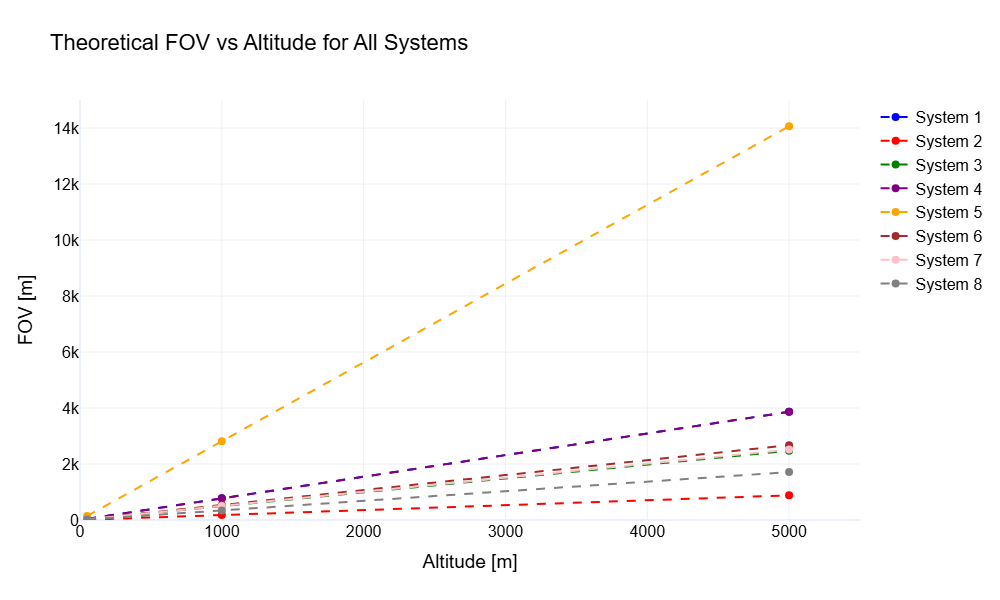
\includegraphics[trim = 0cm 0cm 0cm 2cm, clip, width=0.9\linewidth]{Figures/C2/disenofov.png}
    \caption{Theoretical ground field of view as a function of altitude
             for the eight optical configurations. Greater is better.}
    \label{fig:fov_vs_altitude}
\end{figure}

\begin{figure}[H]
    \centering
    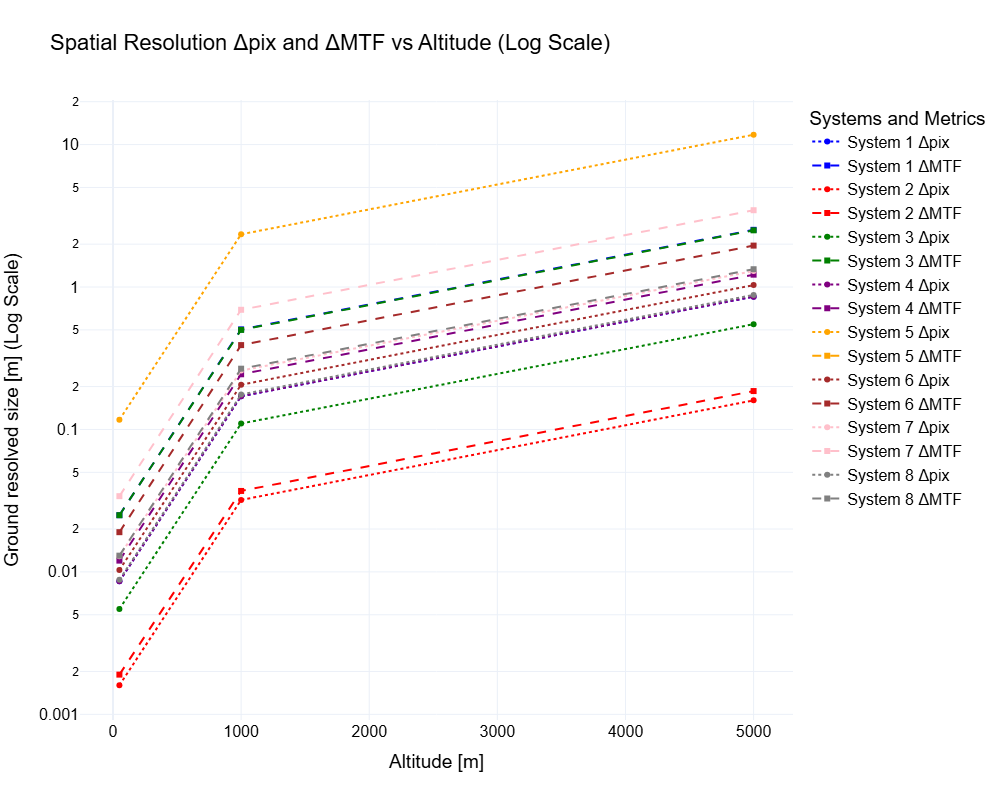
\includegraphics[trim = 0cm 0cm 0cm 2cm, clip, width=0.9\linewidth]{Figures/C2/design_res.png}
    \caption{Ground‐sampled distance determined by the $\approx 30 \%$ MTF
             cut-off (\(\Delta_{\mathrm{MTF}}\)) versus altitude.  System 5
             is omitted because manufacturer data do not report an MTF
             curve for the selected objetive. Less is better.}
    \label{fig:mtf_vs_altitude}
\end{figure}

\noindent At first glance, \(\Delta_{\mathrm{MTF}}\) is always larger than
\(\Delta_{\mathrm{pix}}\), as expected: the optics attenuate high
frequencies and thus slightly limit the detail that the sensor could
ideally capture. This confirms that the chosen pixel sizes are small
enough not to waste lens resolution; indeed, a larger pixel—which may
reduce sensor cost and improve SNR—could be used without losing image
detail, a possibility left for future upgrades.\\


\noindent Regarding the balance between FOV and MTF, long-focal lenses
concentrate each pixel on a reduced area—better sharpness—but restrict
the FOV (e.g.\ system 2 gives an 881 m FOV and 20 cm ground
resolution at 5 km).  Figure~\ref{fig:fov_vs_altitude} every system FOV vs working distance. Such lenses are ideal when high resolution, not coverage, is required—for instance, urban structures or individual
flora /fauna.  Conversely, very short focal lengths greatly expand FOV
at the expense of resolution (system 5: 14 km FOV at 5 km altitude).
These systems are useful when large coverage at close range is needed,
such as surveillance cameras on a mast tens of metres high.\\

\noindent Systems 3 and 4 appear attractive for 5000 m altitude.  System 3 offers
a vertical FOV of 2473 m with 2.5 m ground resolution, whereas system 4
provides 3863 m FOV with 1.2 m resolution. Both, however, rely on a
12.36 × 12.36 mm, 20 MP sensor costing USD 2500—clearly over-specified
for the selected lenses and pushing total costs to USD 3379 and
USD 3550, respectively, while adding considerable mass (78 g and
128 g).\\

\noindent Given the system requirements, systems 6 and 7 offer the best
compromise: similar optics (8 mm f/2.5 and 8.5 mm f/1.8) yield balanced
coverage and detail. At 50 m altitude, system 6 provides a 26.73 m FOV
with \(\Delta_{\mathrm{MTF}}=1.9\) cm, while system 7 offers a comparable
FOV with \(\Delta_{\mathrm{MTF}}=3.4\) cm. At 1000 m these become 39 cm
and 69 cm, respectively, over $\approx$ 500 m coverage; at 5000 m, FOVs of
$\approx$ 2.7 km and $\approx$ 2.5 km with 2–3.5 m resolution. Their nearly identical
geometry simplifies multispectral fusion and alignment. Moreover, their
costs—USD 541 and USD 777 (sensor + lens)—fit comfortably under the
USD 1500 limit.\\

\subsection{Design-process conclusions}

Considering mass, power, bit depth and pixel size together with the
results of Table~\ref{tab:sensor_table}, the optimal configuration is
the AR0521 (VIS) + AR0522 (NIR) pair mounted on 8 mm f/2.5 and
8.5 mm f/1.8 lenses (systems 6 and 7). This combination delivers an
ideal balance of resolution, field of view and energy efficiency for the
\textit{C3} missions. Funding for systems 6 and 7 was provided by the
4DAir project at Universidad EAFIT, led by Dr.\ Elena Montilla Rosero, as
acknowledged in this thesis.\\

\subsection{Candidate optical systems}% Main appendix title
\label{ap:sistemas_candidatos} 

The following tables summarise all the information for the eight
candidate optical systems:

% (all four large tables remain unchanged, only their captions,
% headings and explanatory text were translated above)


\begin{table}[H]
\centering
\resizebox{\textwidth}{!}{
\begin{tabular}{ccc|cc|cc|}
\cline{4-7}
 &
  \textbf{} &
  \textbf{} &
  \multicolumn{2}{c|}{\textbf{System 1}} &
  \multicolumn{2}{c|}{\textbf{System 2}} \\ \hline
\multicolumn{1}{|c|}{} &
  \multicolumn{2}{c|}{\cellcolor[HTML]{EFEFEF}\textbf{Name}} &
  \multicolumn{2}{c|}{\cellcolor[HTML]{EFEFEF}{\color[HTML]{0563C1} {\ul Alvium 1800 U-2040 | 20.4 MP Sony IMX541 CMOS sensor - Allied Vision}}} &
  \multicolumn{2}{c|}{\cellcolor[HTML]{EFEFEF}{\color[HTML]{0563C1} {\ul Alvium 1800 U-2050}}} \\
\multicolumn{1}{|c|}{} &
  \multicolumn{2}{c|}{\textbf{Tipo}} &
  \multicolumn{2}{c|}{Sony IMX541} &
  \multicolumn{2}{c|}{Sony IMX183} \\
\multicolumn{1}{|c|}{} &
  \multicolumn{2}{c|}{\cellcolor[HTML]{EFEFEF}\textbf{Weight}} &
  \multicolumn{2}{c|}{\cellcolor[HTML]{EFEFEF}65} &
  \multicolumn{2}{c|}{\cellcolor[HTML]{EFEFEF}65} \\
\multicolumn{1}{|c|}{} &
  \multicolumn{2}{c|}{\textbf{Prize}} &
  \multicolumn{2}{c|}{\$2,215.00} &
  \multicolumn{2}{c|}{\$701.00} \\
\multicolumn{1}{|c|}{} &
  \multicolumn{2}{c|}{\cellcolor[HTML]{EFEFEF}\textbf{Sensor size (V) {[}pxiels{]}}} &
  \multicolumn{2}{c|}{\cellcolor[HTML]{EFEFEF}4512} &
  \multicolumn{2}{c|}{\cellcolor[HTML]{EFEFEF}3672} \\
\multicolumn{1}{|c|}{} &
  \multicolumn{2}{c|}{\textbf{Sensor size (H) {[}pxiels{]}}} &
  \multicolumn{2}{c|}{4512} &
  \multicolumn{2}{c|}{5496} \\
\multicolumn{1}{|c|}{} &
  \multicolumn{2}{c|}{\cellcolor[HTML]{EFEFEF}\textbf{Sensor's resolution {[}lp/mm{]}}} &
  \multicolumn{2}{c|}{\cellcolor[HTML]{EFEFEF}182,4817518} &
  \multicolumn{2}{c|}{\cellcolor[HTML]{EFEFEF}208,3333333} \\
\multicolumn{1}{|c|}{} &
  \multicolumn{2}{c|}{\textbf{Pixel size {[}µm {]}}} &
  \multicolumn{2}{c|}{2,74} &
  \multicolumn{2}{c|}{2,4} \\
\multicolumn{1}{|c|}{} &
  \multicolumn{2}{c|}{\cellcolor[HTML]{EFEFEF}\textbf{Physical size Height (mm)}} &
  \multicolumn{2}{c|}{\cellcolor[HTML]{EFEFEF}12,36288} &
  \multicolumn{2}{c|}{\cellcolor[HTML]{EFEFEF}8,8128} \\
\multicolumn{1}{|c|}{} &
  \multicolumn{2}{c|}{\textbf{Physical size Width  (mm)}} &
  \multicolumn{2}{c|}{12,36288} &
  \multicolumn{2}{c|}{13,1904} \\
\multicolumn{1}{|c|}{} &
  \multicolumn{2}{c|}{\cellcolor[HTML]{EFEFEF}\textbf{Color}} &
  \multicolumn{2}{c|}{\cellcolor[HTML]{EFEFEF}BW and Color} &
  \multicolumn{2}{c|}{\cellcolor[HTML]{EFEFEF}BW and Color} \\
\multicolumn{1}{|c|}{} &
  \multicolumn{2}{c|}{\textbf{Operational temperature}} &
  \multicolumn{2}{c|}{-20 -\textgreater 65 C°} &
  \multicolumn{2}{c|}{-20 -\textgreater 65C°} \\
\multicolumn{1}{|c|}{} &
  \multicolumn{2}{c|}{\cellcolor[HTML]{EFEFEF}\textbf{Spectral range}} &
  \multicolumn{2}{c|}{\cellcolor[HTML]{EFEFEF}300 to 1100 nm} &
  \multicolumn{2}{c|}{\cellcolor[HTML]{EFEFEF}300 to 1100 nm} \\
\multicolumn{1}{|c|}{} &
  \multicolumn{2}{c|}{\textbf{Sensor type}} &
  \multicolumn{2}{c|}{CMOS} &
  \multicolumn{2}{c|}{CMOS} \\
\multicolumn{1}{|c|}{} &
  \multicolumn{2}{c|}{\cellcolor[HTML]{EFEFEF}\textbf{Lens mount}} &
  \multicolumn{2}{c|}{\cellcolor[HTML]{EFEFEF}C-Mount, CS-Mount} &
  \multicolumn{2}{c|}{\cellcolor[HTML]{EFEFEF}C-Mount} \\
\multicolumn{1}{|c|}{} &
  \multicolumn{2}{c|}{\textbf{Max. fram rate at full resolution}} &
  \multicolumn{2}{c|}{21 fps at 450 MByte/s, Mono8} &
  \multicolumn{2}{c|}{21 fps at 450 MByte/s, Mono8} \\
\multicolumn{1}{|c|}{} &
  \multicolumn{2}{c|}{\cellcolor[HTML]{EFEFEF}\textbf{ADC}} &
  \multicolumn{2}{c|}{\cellcolor[HTML]{EFEFEF}12 Bit} &
  \multicolumn{2}{c|}{\cellcolor[HTML]{EFEFEF}12 Bit} \\
\multicolumn{1}{|c|}{} &
  \multicolumn{2}{c|}{\textbf{Image buffer (RAM)}} &
  \multicolumn{2}{c|}{256 KByte} &
  \multicolumn{2}{c|}{256 KByte} \\
\multicolumn{1}{|c|}{} &
  \multicolumn{2}{c|}{\cellcolor[HTML]{EFEFEF}\textbf{Bit depth}} &
  \multicolumn{2}{c|}{\cellcolor[HTML]{EFEFEF}12-bit Bit} &
  \multicolumn{2}{c|}{\cellcolor[HTML]{EFEFEF}10-bit Bit} \\
\multicolumn{1}{|c|}{} &
  \multicolumn{2}{c|}{\textbf{Physical characteristics : Dimensions}} &
  \multicolumn{2}{c|}{29.4 x 29.4 x 38.2 mm} &
  \multicolumn{2}{c|}{38 $\times$ 29 $\times$ 29} \\
\multicolumn{1}{|c|}{} &
  \multicolumn{2}{c|}{\cellcolor[HTML]{EFEFEF}\textbf{Power requirements (DC)}} &
  \multicolumn{2}{c|}{\cellcolor[HTML]{EFEFEF}Power over USB 3.1 Gen 1 | External power 5.0 V} &
  \multicolumn{2}{c|}{\cellcolor[HTML]{EFEFEF}Power over USB 3.1 Gen 1 | External power 5.0 V} \\
\multicolumn{1}{|c|}{\multirow{-22}{*}{\textbf{Sensor}}} &
  \multicolumn{2}{c|}{\textbf{Power consumption}} &
  \multicolumn{2}{c|}{USB power: 3.9 W (typical) | Ext. power: 4.1 W (typical)} &
  \multicolumn{2}{c|}{USB power: 3.2 W (typical) | Ext. power: 3.4 W (typical)} \\ \hline
\multicolumn{1}{|c|}{} &
  \multicolumn{2}{c|}{\cellcolor[HTML]{EFEFEF}\textbf{Name}} &
  \multicolumn{2}{c|}{\cellcolor[HTML]{EFEFEF}{\color[HTML]{0563C1} {\ul 16mm f/16, HPr Series Fixed Focal Length Lens | Edmund Optics}}} &
  \multicolumn{2}{c|}{\cellcolor[HTML]{EFEFEF}{\color[HTML]{0563C1} {\ul 50mm f/2.8, HPr Series Fixed Focal Length Lens}}} \\
\multicolumn{1}{|c|}{} &
  \multicolumn{2}{c|}{\textbf{Focal distance {[}mm{]}}} &
  \multicolumn{2}{c|}{16} &
  \multicolumn{2}{c|}{50} \\
\multicolumn{1}{|c|}{} &
  \multicolumn{2}{c|}{\cellcolor[HTML]{EFEFEF}\textbf{AFOV}} &
  \multicolumn{2}{c|}{\cellcolor[HTML]{EFEFEF}0,737350672} &
  \multicolumn{2}{c|}{\cellcolor[HTML]{EFEFEF}0,175801815} \\
\multicolumn{1}{|c|}{} &
  \multicolumn{2}{c|}{\textbf{Aperture}} &
  \multicolumn{2}{c|}{f/16} &
  \multicolumn{2}{c|}{f/2,8} \\
\multicolumn{1}{|c|}{} &
  \multicolumn{2}{c|}{\cellcolor[HTML]{EFEFEF}\textbf{Weight {[}g{]}}} &
  \multicolumn{2}{c|}{\cellcolor[HTML]{EFEFEF}138} &
  \multicolumn{2}{c|}{\cellcolor[HTML]{EFEFEF}No specified} \\
\multicolumn{1}{|c|}{\multirow{-6}{*}{\textbf{Lens}}} &
  \multicolumn{2}{c|}{\textbf{MTF at 30\% contrast {[}lp / mm{]}}} &
  \multicolumn{2}{c|}{62} &
  \multicolumn{2}{c|}{180} \\ \hline
\multicolumn{1}{|c|}{} &
  \multicolumn{2}{c|}{\cellcolor[HTML]{EFEFEF}\textbf{Name}} &
  \multicolumn{2}{c|}{\cellcolor[HTML]{EFEFEF}Raspberry Pi 4} &
  \multicolumn{2}{c|}{\cellcolor[HTML]{EFEFEF}Raspberry Pi 4} \\
\multicolumn{1}{|c|}{\multirow{-2}{*}{\textbf{\begin{tabular}[c]{@{}c@{}}Graphics \\ processor\end{tabular}}}} &
  \multicolumn{2}{c|}{\textbf{Weight {[}g{]}}} &
  \multicolumn{2}{c|}{46} &
  \multicolumn{2}{c|}{46 g} \\ \hline
\multicolumn{1}{|c|}{} &
  \cellcolor[HTML]{EFEFEF} &
  \cellcolor[HTML]{EFEFEF} &
  \cellcolor[HTML]{EFEFEF}Fov {[}m{]} &
  \cellcolor[HTML]{EFEFEF}38,634 &
  \cellcolor[HTML]{EFEFEF}Fov {[}m{]} &
  \cellcolor[HTML]{EFEFEF}8,8128 \\
\multicolumn{1}{|c|}{} &
  \cellcolor[HTML]{EFEFEF} &
  \cellcolor[HTML]{EFEFEF} &
  Magnification &
  0,00032 &
  Magnification &
  0,001496732 \\
\multicolumn{1}{|c|}{} &
  \cellcolor[HTML]{EFEFEF} &
  \cellcolor[HTML]{EFEFEF} &
  \cellcolor[HTML]{EFEFEF}Resolution object plane {[}m{]} &
  \cellcolor[HTML]{EFEFEF}0,0085625 &
  \cellcolor[HTML]{EFEFEF}Resolution object plane {[}m{]} &
  \cellcolor[HTML]{EFEFEF}0,001603493 \\
\multicolumn{1}{|c|}{} &
  \multirow{-4}{*}{\cellcolor[HTML]{EFEFEF}\textbf{50}} &
  \multirow{-4}{*}{\cellcolor[HTML]{EFEFEF}\textbf{m}} &
  Resolution object plane with lens' MTF at 30 \% contrast {[}m{]} &
  0,025201613 &
  Resolution object plane with lens' MTF at 30 \% contrast {[}m{]} &
  0,001855895 \\ \cline{2-7} 
\multicolumn{1}{|c|}{} &
  \cellcolor[HTML]{EFEFEF} &
  \cellcolor[HTML]{EFEFEF} &
  \cellcolor[HTML]{EFEFEF}Fov {[}m{]} &
  \cellcolor[HTML]{EFEFEF}772,68 &
  \cellcolor[HTML]{EFEFEF}Fov {[}m{]} &
  \cellcolor[HTML]{EFEFEF}176,256 \\
\multicolumn{1}{|c|}{} &
  \cellcolor[HTML]{EFEFEF} &
  \cellcolor[HTML]{EFEFEF} &
  Magnification &
  0,000016 &
  Magnification &
  7,48366E-05 \\
\multicolumn{1}{|c|}{} &
  \cellcolor[HTML]{EFEFEF} &
  \cellcolor[HTML]{EFEFEF} &
  \cellcolor[HTML]{EFEFEF}Resolution object plane {[}m{]} &
  \cellcolor[HTML]{EFEFEF}0,17125 &
  \cellcolor[HTML]{EFEFEF}Resolution object plane {[}m{]} &
  \cellcolor[HTML]{EFEFEF}0,032069869 \\
\multicolumn{1}{|c|}{} &
  \multirow{-4}{*}{\cellcolor[HTML]{EFEFEF}\textbf{1000}} &
  \multirow{-4}{*}{\cellcolor[HTML]{EFEFEF}\textbf{m}} &
  Resolution object plane with lens' MTF at 30 \% contrast {[}m{]} &
  0,504032258 &
  Resolution object plane with lens' MTF at 30 \% contrast {[}m{]} &
  0,037117904 \\ \cline{2-7} 
\multicolumn{1}{|c|}{} &
  \cellcolor[HTML]{EFEFEF} &
  \cellcolor[HTML]{EFEFEF} &
  \cellcolor[HTML]{EFEFEF}Fov {[}m{]} &
  \cellcolor[HTML]{EFEFEF}3863,4 &
  \cellcolor[HTML]{EFEFEF}Fov {[}m{]} &
  \cellcolor[HTML]{EFEFEF}881,28 \\
\multicolumn{1}{|c|}{} &
  \cellcolor[HTML]{EFEFEF} &
  \cellcolor[HTML]{EFEFEF} &
  Magnification &
  0,0000032 &
  Magnification &
  1,49673E-05 \\
\multicolumn{1}{|c|}{} &
  \cellcolor[HTML]{EFEFEF} &
  \cellcolor[HTML]{EFEFEF} &
  \cellcolor[HTML]{EFEFEF}Resolution object plane {[}m{]} &
  \cellcolor[HTML]{EFEFEF}0,85625 &
  \cellcolor[HTML]{EFEFEF}Resolution object plane {[}m{]} &
  \cellcolor[HTML]{EFEFEF}0,160349345 \\
\multicolumn{1}{|c|}{\multirow{-12}{*}{\textbf{\begin{tabular}[c]{@{}c@{}}Ground resolution \\ and field of view\\ with a x \\ working distance\end{tabular}}}} &
  \multirow{-4}{*}{\cellcolor[HTML]{EFEFEF}\textbf{5000}} &
  \multirow{-4}{*}{\cellcolor[HTML]{EFEFEF}\textbf{m}} &
  Resolution object plane with lens' MTF at 30 \% contrast {[}m{]} &
  2,52016129 &
  Resolution object plane with lens' MTF at 30 \% contrast {[}m{]} &
  0,18558952 \\ \hline
\end{tabular}
}
\end{table}


\begin{table}[H]
\centering
\resizebox{\textwidth}{!}{%
\begin{tabular}{ccc|cc|cc|}
\cline{4-7}
 &
  \textbf{} &
  \textbf{} &
  \multicolumn{2}{c|}{\textbf{System 3}} &
  \multicolumn{2}{c|}{\textbf{System 4}} \\ \hline
\multicolumn{1}{|c|}{} &
  \multicolumn{2}{c|}{\cellcolor[HTML]{EFEFEF}\textbf{Name}} &
  \multicolumn{2}{c|}{\cellcolor[HTML]{EFEFEF}{\color[HTML]{0563C1} {\ul Alvium 1800 U-2040 | 20.4 MP Sony IMX541 CMOS sensor - Allied Vision}}} &
  \multicolumn{2}{c|}{\cellcolor[HTML]{EFEFEF}{\color[HTML]{0563C1} {\ul Alvium 1800 U-2040 | 20.4 MP Sony IMX541 CMOS sensor - Allied Vision}}} \\
\multicolumn{1}{|c|}{} &
  \multicolumn{2}{c|}{\textbf{Tipo}} &
  \multicolumn{2}{c|}{Sony IMX541} &
  \multicolumn{2}{c|}{Sony IMX541} \\
\multicolumn{1}{|c|}{} &
  \multicolumn{2}{c|}{\cellcolor[HTML]{EFEFEF}\textbf{Weight}} &
  \multicolumn{2}{c|}{\cellcolor[HTML]{EFEFEF}65} &
  \multicolumn{2}{c|}{\cellcolor[HTML]{EFEFEF}65} \\
\multicolumn{1}{|c|}{} &
  \multicolumn{2}{c|}{\textbf{Prize}} &
  \multicolumn{2}{c|}{\$2,215.00} &
  \multicolumn{2}{c|}{\$2,215.00} \\
\multicolumn{1}{|c|}{} &
  \multicolumn{2}{c|}{\cellcolor[HTML]{EFEFEF}\textbf{Sensor size (V) {[}pxiels{]}}} &
  \multicolumn{2}{c|}{\cellcolor[HTML]{EFEFEF}4512} &
  \multicolumn{2}{c|}{\cellcolor[HTML]{EFEFEF}4512} \\
\multicolumn{1}{|c|}{} &
  \multicolumn{2}{c|}{\textbf{Sensor size (H) {[}pxiels{]}}} &
  \multicolumn{2}{c|}{4512} &
  \multicolumn{2}{c|}{4512} \\
\multicolumn{1}{|c|}{} &
  \multicolumn{2}{c|}{\cellcolor[HTML]{EFEFEF}\textbf{Sensor's resolution {[}lp/mm{]}}} &
  \multicolumn{2}{c|}{\cellcolor[HTML]{EFEFEF}182,4817518} &
  \multicolumn{2}{c|}{\cellcolor[HTML]{EFEFEF}182,4817518} \\
\multicolumn{1}{|c|}{} &
  \multicolumn{2}{c|}{\textbf{Pixel size {[}µm {]}}} &
  \multicolumn{2}{c|}{2,74} &
  \multicolumn{2}{c|}{2,74} \\
\multicolumn{1}{|c|}{} &
  \multicolumn{2}{c|}{\cellcolor[HTML]{EFEFEF}\textbf{Physical size Height (mm)}} &
  \multicolumn{2}{c|}{\cellcolor[HTML]{EFEFEF}12,36288} &
  \multicolumn{2}{c|}{\cellcolor[HTML]{EFEFEF}12,36288} \\
\multicolumn{1}{|c|}{} &
  \multicolumn{2}{c|}{\textbf{Physical size Width  (mm)}} &
  \multicolumn{2}{c|}{12,36288} &
  \multicolumn{2}{c|}{12,36288} \\
\multicolumn{1}{|c|}{} &
  \multicolumn{2}{c|}{\cellcolor[HTML]{EFEFEF}\textbf{Color}} &
  \multicolumn{2}{c|}{\cellcolor[HTML]{EFEFEF}BW and Color} &
  \multicolumn{2}{c|}{\cellcolor[HTML]{EFEFEF}BW and Color} \\
\multicolumn{1}{|c|}{} &
  \multicolumn{2}{c|}{\textbf{Operational temperature}} &
  \multicolumn{2}{c|}{-20 -\textgreater 65 C°} &
  \multicolumn{2}{c|}{-20 -\textgreater 65 C°} \\
\multicolumn{1}{|c|}{} &
  \multicolumn{2}{c|}{\cellcolor[HTML]{EFEFEF}\textbf{Spectral range}} &
  \multicolumn{2}{c|}{\cellcolor[HTML]{EFEFEF}300 to 1100 nm} &
  \multicolumn{2}{c|}{\cellcolor[HTML]{EFEFEF}300 to 1100 nm} \\
\multicolumn{1}{|c|}{} &
  \multicolumn{2}{c|}{\textbf{Sensor type}} &
  \multicolumn{2}{c|}{CMOS} &
  \multicolumn{2}{c|}{CMOS} \\
\multicolumn{1}{|c|}{} &
  \multicolumn{2}{c|}{\cellcolor[HTML]{EFEFEF}\textbf{Lens mount}} &
  \multicolumn{2}{c|}{\cellcolor[HTML]{EFEFEF}C-Mount, CS-Mount} &
  \multicolumn{2}{c|}{\cellcolor[HTML]{EFEFEF}C-Mount, CS-Mount} \\
\multicolumn{1}{|c|}{} &
  \multicolumn{2}{c|}{\textbf{Max. fram rate at full resolution}} &
  \multicolumn{2}{c|}{21 fps at 450 MByte/s, Mono8} &
  \multicolumn{2}{c|}{21 fps at 450 MByte/s, Mono8} \\
\multicolumn{1}{|c|}{} &
  \multicolumn{2}{c|}{\cellcolor[HTML]{EFEFEF}\textbf{ADC}} &
  \multicolumn{2}{c|}{\cellcolor[HTML]{EFEFEF}12 Bit} &
  \multicolumn{2}{c|}{\cellcolor[HTML]{EFEFEF}12 Bit} \\
\multicolumn{1}{|c|}{} &
  \multicolumn{2}{c|}{\textbf{Image buffer (RAM)}} &
  \multicolumn{2}{c|}{256 KByte} &
  \multicolumn{2}{c|}{256 KByte} \\
\multicolumn{1}{|c|}{} &
  \multicolumn{2}{c|}{\cellcolor[HTML]{EFEFEF}\textbf{Bit depth}} &
  \multicolumn{2}{c|}{\cellcolor[HTML]{EFEFEF}12-bit Bit} &
  \multicolumn{2}{c|}{\cellcolor[HTML]{EFEFEF}12-bit Bit} \\
\multicolumn{1}{|c|}{} &
  \multicolumn{2}{c|}{\textbf{Physical characteristics : Dimensions}} &
  \multicolumn{2}{c|}{26 x 29 x 29} &
  \multicolumn{2}{c|}{29.4 x 29.4 x 38.2 mm} \\
\multicolumn{1}{|c|}{} &
  \multicolumn{2}{c|}{\cellcolor[HTML]{EFEFEF}\textbf{Power requirements (DC)}} &
  \multicolumn{2}{c|}{\cellcolor[HTML]{EFEFEF}5 VDC over MIPI CSI-2} &
  \multicolumn{2}{c|}{\cellcolor[HTML]{EFEFEF}Power over USB 3.1 Gen 1 | External power 5.0 V} \\
\multicolumn{1}{|c|}{\multirow{-22}{*}{\textbf{Sensor}}} &
  \multicolumn{2}{c|}{\textbf{Power consumption}} &
  \multicolumn{2}{c|}{Typical: 3.7 W} &
  \multicolumn{2}{c|}{USB power: 3.9 W (typical) | Ext. power: 4.1 W (typical)} \\ \hline
\multicolumn{1}{|c|}{} &
  \multicolumn{2}{c|}{\cellcolor[HTML]{EFEFEF}\textbf{Name}} &
  \multicolumn{2}{c|}{\cellcolor[HTML]{EFEFEF}{\color[HTML]{0563C1} {\ul 25mm f/1.8, HPr Series Fixed Focal Length Lens}}} &
  \multicolumn{2}{c|}{\cellcolor[HTML]{EFEFEF}{\color[HTML]{0563C1} {\ul 16mm f/1.8, HPr Series Fixed Focal Length Lens}}} \\
\multicolumn{1}{|c|}{} &
  \multicolumn{2}{c|}{\textbf{Focal distance {[}mm{]}}} &
  \multicolumn{2}{c|}{25} &
  \multicolumn{2}{c|}{16} \\
\multicolumn{1}{|c|}{} &
  \multicolumn{2}{c|}{\cellcolor[HTML]{EFEFEF}\textbf{AFOV}} &
  \multicolumn{2}{c|}{\cellcolor[HTML]{EFEFEF}0,48479184} &
  \multicolumn{2}{c|}{\cellcolor[HTML]{EFEFEF}0,737350672} \\
\multicolumn{1}{|c|}{} &
  \multicolumn{2}{c|}{\textbf{Aperture}} &
  \multicolumn{2}{c|}{f/1,8} &
  \multicolumn{2}{c|}{f/1,8} \\
\multicolumn{1}{|c|}{} &
  \multicolumn{2}{c|}{\cellcolor[HTML]{EFEFEF}\textbf{Weight {[}g{]}}} &
  \multicolumn{2}{c|}{\cellcolor[HTML]{EFEFEF}78} &
  \multicolumn{2}{c|}{\cellcolor[HTML]{EFEFEF}{\color[HTML]{333333} 138}} \\
\multicolumn{1}{|c|}{\multirow{-6}{*}{\textbf{Lens}}} &
  \multicolumn{2}{c|}{\textbf{MTF at 30\% contrast {[}lp / mm{]}}} &
  \multicolumn{2}{c|}{40} &
  \multicolumn{2}{c|}{128} \\ \hline
\multicolumn{1}{|c|}{} &
  \multicolumn{2}{c|}{\cellcolor[HTML]{EFEFEF}\textbf{Name}} &
  \multicolumn{2}{c|}{\cellcolor[HTML]{EFEFEF}Raspberry Pi 4} &
  \multicolumn{2}{c|}{\cellcolor[HTML]{EFEFEF}Raspberry Pi 4} \\
\multicolumn{1}{|c|}{\multirow{-2}{*}{\textbf{\begin{tabular}[c]{@{}c@{}}Graphics \\ processor\end{tabular}}}} &
  \multicolumn{2}{c|}{\textbf{Weight {[}g{]}}} &
  \multicolumn{2}{c|}{46} &
  \multicolumn{2}{c|}{46} \\ \hline
\multicolumn{1}{|c|}{} &
  \cellcolor[HTML]{EFEFEF} &
  \cellcolor[HTML]{EFEFEF} &
  \cellcolor[HTML]{EFEFEF}Fov {[}m{]} &
  \cellcolor[HTML]{EFEFEF}24,72576 &
  \cellcolor[HTML]{EFEFEF}Fov {[}m{]} &
  \cellcolor[HTML]{EFEFEF}38,634 \\
\multicolumn{1}{|c|}{} &
  \cellcolor[HTML]{EFEFEF} &
  \cellcolor[HTML]{EFEFEF} &
  Magnification &
  0,0005 &
  Magnification &
  0,00032 \\
\multicolumn{1}{|c|}{} &
  \cellcolor[HTML]{EFEFEF} &
  \cellcolor[HTML]{EFEFEF} &
  \cellcolor[HTML]{EFEFEF}Resolution object plane {[}m{]} &
  \cellcolor[HTML]{EFEFEF}0,00548 &
  \cellcolor[HTML]{EFEFEF}Resolution object plane {[}m{]} &
  \cellcolor[HTML]{EFEFEF}0,0085625 \\
\multicolumn{1}{|c|}{} &
  \multirow{-4}{*}{\cellcolor[HTML]{EFEFEF}\textbf{50}} &
  \multirow{-4}{*}{\cellcolor[HTML]{EFEFEF}\textbf{m}} &
  Resolution object plane with lens' MTF at 30 \% contrast {[}m{]} &
  0,025 &
  Resolution object plane with lens' MTF at 30 \% contrast {[}m{]} &
  0,012207031 \\ \cline{2-7} 
\multicolumn{1}{|c|}{} &
  \cellcolor[HTML]{EFEFEF} &
  \cellcolor[HTML]{EFEFEF} &
  \cellcolor[HTML]{EFEFEF}Fov {[}m{]} &
  \cellcolor[HTML]{EFEFEF}494,5152 &
  \cellcolor[HTML]{EFEFEF}Fov {[}m{]} &
  \cellcolor[HTML]{EFEFEF}772,68 \\
\multicolumn{1}{|c|}{} &
  \cellcolor[HTML]{EFEFEF} &
  \cellcolor[HTML]{EFEFEF} &
  Magnification &
  0,000025 &
  Magnification &
  0,000016 \\
\multicolumn{1}{|c|}{} &
  \cellcolor[HTML]{EFEFEF} &
  \cellcolor[HTML]{EFEFEF} &
  \cellcolor[HTML]{EFEFEF}Resolution object plane {[}m{]} &
  \cellcolor[HTML]{EFEFEF}0,1096 &
  \cellcolor[HTML]{EFEFEF}Resolution object plane {[}m{]} &
  \cellcolor[HTML]{EFEFEF}0,17125 \\
\multicolumn{1}{|c|}{} &
  \multirow{-4}{*}{\cellcolor[HTML]{EFEFEF}\textbf{1000}} &
  \multirow{-4}{*}{\cellcolor[HTML]{EFEFEF}\textbf{m}} &
  Resolution object plane with lens' MTF at 30 \% contrast {[}m{]} &
  0,5 &
  Resolution object plane with lens' MTF at 30 \% contrast {[}m{]} &
  0,244140625 \\ \cline{2-7} 
\multicolumn{1}{|c|}{} &
  \cellcolor[HTML]{EFEFEF} &
  \cellcolor[HTML]{EFEFEF} &
  \cellcolor[HTML]{EFEFEF}Fov {[}m{]} &
  \cellcolor[HTML]{EFEFEF}2472,576 &
  \cellcolor[HTML]{EFEFEF}Fov {[}m{]} &
  \cellcolor[HTML]{EFEFEF}3863,4 \\
\multicolumn{1}{|c|}{} &
  \cellcolor[HTML]{EFEFEF} &
  \cellcolor[HTML]{EFEFEF} &
  Magnification &
  0,000005 &
  Magnification &
  0,0000032 \\
\multicolumn{1}{|c|}{} &
  \cellcolor[HTML]{EFEFEF} &
  \cellcolor[HTML]{EFEFEF} &
  \cellcolor[HTML]{EFEFEF}Resolution object plane {[}m{]} &
  \cellcolor[HTML]{EFEFEF}0,548 &
  \cellcolor[HTML]{EFEFEF}Resolution object plane {[}m{]} &
  \cellcolor[HTML]{EFEFEF}0,85625 \\
\multicolumn{1}{|c|}{\multirow{-12}{*}{\textbf{\begin{tabular}[c]{@{}c@{}}Ground resolution \\ and field of view\\ with a x \\ working distance\end{tabular}}}} &
  \multirow{-4}{*}{\cellcolor[HTML]{EFEFEF}\textbf{5000}} &
  \multirow{-4}{*}{\cellcolor[HTML]{EFEFEF}\textbf{m}} &
  Resolution object plane with lens' MTF at 30 \% contrast {[}m{]} &
  2,5 &
  Resolution object plane with lens' MTF at 30 \% contrast {[}m{]} &
  1,220703125 \\ \hline
\end{tabular}%
}
\end{table}


\begin{table}[H]
\centering
\resizebox{\textwidth}{!}{%
\begin{tabular}{ccc|cc|cc|}
\cline{4-7}
 &
  \textbf{} &
  \textbf{} &
  \multicolumn{2}{c|}{\textbf{System 5}} &
  \multicolumn{2}{c|}{\textbf{System 6 (NIR)}} \\ \hline
\multicolumn{1}{|c|}{} &
  \multicolumn{2}{c|}{\cellcolor[HTML]{EFEFEF}\textbf{Name}} &
  \multicolumn{2}{c|}{\cellcolor[HTML]{EFEFEF}{\color[HTML]{0563C1} {\ul Basler ace acA1920-40gc - Area Scan Camera (baslerweb.com)}}} &
  \multicolumn{2}{c|}{\cellcolor[HTML]{EFEFEF}{\color[HTML]{0563C1} {\ul Allied Vision Alvium 1800 U-501m NIR, 1/2.5" 5MP S-Mount, Right Angle USB 3.1 NIR Camera}}} \\
\multicolumn{1}{|c|}{} &
  \multicolumn{2}{c|}{\textbf{Tipo}} &
  \multicolumn{2}{c|}{IMX249} &
  \multicolumn{2}{c|}{ON Semi AR0522} \\
\multicolumn{1}{|c|}{} &
  \multicolumn{2}{c|}{\cellcolor[HTML]{EFEFEF}\textbf{Weight}} &
  \multicolumn{2}{c|}{\cellcolor[HTML]{EFEFEF}90} &
  \multicolumn{2}{c|}{\cellcolor[HTML]{EFEFEF}65} \\
\multicolumn{1}{|c|}{} &
  \multicolumn{2}{c|}{\textbf{Prize}} &
  \multicolumn{2}{c|}{\$670.00} &
  \multicolumn{2}{c|}{\$351.00} \\
\multicolumn{1}{|c|}{} &
  \multicolumn{2}{c|}{\cellcolor[HTML]{EFEFEF}\textbf{Sensor size (V) {[}pxiels{]}}} &
  \multicolumn{2}{c|}{\cellcolor[HTML]{EFEFEF}1920} &
  \multicolumn{2}{c|}{\cellcolor[HTML]{EFEFEF}1944} \\
\multicolumn{1}{|c|}{} &
  \multicolumn{2}{c|}{\textbf{Sensor size (H) {[}pxiels{]}}} &
  \multicolumn{2}{c|}{1200} &
  \multicolumn{2}{c|}{2592} \\
\multicolumn{1}{|c|}{} &
  \multicolumn{2}{c|}{\cellcolor[HTML]{EFEFEF}\textbf{Sensor's resolution {[}lp/mm{]}}} &
  \multicolumn{2}{c|}{\cellcolor[HTML]{EFEFEF}85,32423208} &
  \multicolumn{2}{c|}{\cellcolor[HTML]{EFEFEF}227,2727273} \\
\multicolumn{1}{|c|}{} &
  \multicolumn{2}{c|}{\textbf{Pixel size {[}µm {]}}} &
  \multicolumn{2}{c|}{5,86} &
  \multicolumn{2}{c|}{2,2} \\
\multicolumn{1}{|c|}{} &
  \multicolumn{2}{c|}{\cellcolor[HTML]{EFEFEF}\textbf{Physical size Height (mm)}} &
  \multicolumn{2}{c|}{\cellcolor[HTML]{EFEFEF}11,2512} &
  \multicolumn{2}{c|}{\cellcolor[HTML]{EFEFEF}4,2768} \\
\multicolumn{1}{|c|}{} &
  \multicolumn{2}{c|}{\textbf{Physical size Width  (mm)}} &
  \multicolumn{2}{c|}{7,032} &
  \multicolumn{2}{c|}{5,7024} \\
\multicolumn{1}{|c|}{} &
  \multicolumn{2}{c|}{\cellcolor[HTML]{EFEFEF}\textbf{Color}} &
  \multicolumn{2}{c|}{\cellcolor[HTML]{EFEFEF}BW and Color} &
  \multicolumn{2}{c|}{\cellcolor[HTML]{EFEFEF}NIRm} \\
\multicolumn{1}{|c|}{} &
  \multicolumn{2}{c|}{\textbf{Operational temperature}} &
  \multicolumn{2}{c|}{0 -\textgreater 50 C°} &
  \multicolumn{2}{c|}{+5 to +65} \\
\multicolumn{1}{|c|}{} &
  \multicolumn{2}{c|}{\cellcolor[HTML]{EFEFEF}\textbf{Spectral range}} &
  \multicolumn{2}{c|}{\cellcolor[HTML]{EFEFEF}300 to 1100 nm} &
  \multicolumn{2}{c|}{\cellcolor[HTML]{EFEFEF}300 to 1100 nm} \\
\multicolumn{1}{|c|}{} &
  \multicolumn{2}{c|}{\textbf{Sensor type}} &
  \multicolumn{2}{c|}{CMOS} &
  \multicolumn{2}{c|}{CMOS} \\
\multicolumn{1}{|c|}{} &
  \multicolumn{2}{c|}{\cellcolor[HTML]{EFEFEF}\textbf{Lens mount}} &
  \multicolumn{2}{c|}{\cellcolor[HTML]{EFEFEF}C-Mount, CS-Mount} &
  \multicolumn{2}{c|}{\cellcolor[HTML]{EFEFEF}C-Mount, CS-Mount, S-Mount} \\
\multicolumn{1}{|c|}{} &
  \multicolumn{2}{c|}{\textbf{Max. fram rate at full resolution}} &
  \multicolumn{2}{c|}{42 fps} &
  \multicolumn{2}{c|}{68 fps at $\geq$350 MByte/s, Mono8} \\
\multicolumn{1}{|c|}{} &
  \multicolumn{2}{c|}{\cellcolor[HTML]{EFEFEF}\textbf{ADC}} &
  \multicolumn{2}{c|}{\cellcolor[HTML]{EFEFEF}12 Bit} &
  \multicolumn{2}{c|}{\cellcolor[HTML]{EFEFEF}10 Bit} \\
\multicolumn{1}{|c|}{} &
  \multicolumn{2}{c|}{\textbf{Image buffer (RAM)}} &
  \multicolumn{2}{c|}{256 KByte} &
  \multicolumn{2}{c|}{256 KByte} \\
\multicolumn{1}{|c|}{} &
  \multicolumn{2}{c|}{\cellcolor[HTML]{EFEFEF}\textbf{Bit depth}} &
  \multicolumn{2}{c|}{\cellcolor[HTML]{EFEFEF}10/12 bits} &
  \multicolumn{2}{c|}{\cellcolor[HTML]{EFEFEF}Max. 10 Bit} \\
\multicolumn{1}{|c|}{} &
  \multicolumn{2}{c|}{\textbf{Physical characteristics : Dimensions}} &
  \multicolumn{2}{c|}{42 mm x 29 mm x 29 mm} &
  \multicolumn{2}{c|}{33 $\times$ 32 $\times$ 29} \\
\multicolumn{1}{|c|}{} &
  \multicolumn{2}{c|}{\cellcolor[HTML]{EFEFEF}\textbf{Power requirements (DC)}} &
  \multicolumn{2}{c|}{\cellcolor[HTML]{EFEFEF}Power over USB 3.1 Gen 1 | External power 5.0 V} &
  \multicolumn{2}{c|}{\cellcolor[HTML]{EFEFEF}Power over USB 3.1 Gen 1 | External power 5.0 V} \\
\multicolumn{1}{|c|}{\multirow{-22}{*}{\textbf{Sensor}}} &
  \multicolumn{2}{c|}{\textbf{Power consumption}} &
  \multicolumn{2}{c|}{USB power: 3.9 W (typical) | Ext. power: 4.1 W (typical)} &
  \multicolumn{2}{c|}{USB power: 2.2 W (typical) | Ext. power: 2.4 W (typical)} \\ \hline
\multicolumn{1}{|c|}{} &
  \multicolumn{2}{c|}{\cellcolor[HTML]{EFEFEF}\textbf{Name}} &
  \multicolumn{2}{c|}{\cellcolor[HTML]{EFEFEF}{\color[HTML]{0563C1} {\ul Basler Lens C125-0418-5M-P f4mm - Lens (baslerweb.com)}}} &
  \multicolumn{2}{c|}{\cellcolor[HTML]{EFEFEF}{\color[HTML]{0563C1} {\ul f/2.5, NIR, 8.0mm HEO Series M12 Lens}}} \\
\multicolumn{1}{|c|}{} &
  \multicolumn{2}{c|}{\textbf{Focal distance {[}mm{]}}} &
  \multicolumn{2}{c|}{4} &
  \multicolumn{2}{c|}{8} \\
\multicolumn{1}{|c|}{} &
  \multicolumn{2}{c|}{\cellcolor[HTML]{EFEFEF}\textbf{AFOV}} &
  \multicolumn{2}{c|}{\cellcolor[HTML]{EFEFEF}1,905404949} &
  \multicolumn{2}{c|}{\cellcolor[HTML]{EFEFEF}0,52238717} \\
\multicolumn{1}{|c|}{} &
  \multicolumn{2}{c|}{\textbf{Aperture}} &
  \multicolumn{2}{c|}{f/1.8} &
  \multicolumn{2}{c|}{f/2.5} \\
\multicolumn{1}{|c|}{} &
  \multicolumn{2}{c|}{\cellcolor[HTML]{EFEFEF}\textbf{Weight {[}g{]}}} &
  \multicolumn{2}{c|}{\cellcolor[HTML]{EFEFEF}{\color[HTML]{333333} -}} &
  \multicolumn{2}{c|}{\cellcolor[HTML]{EFEFEF}{\color[HTML]{333333} 4}} \\
\multicolumn{1}{|c|}{\multirow{-6}{*}{\textbf{Lens}}} &
  \multicolumn{2}{c|}{\textbf{MTF at 30\% contrast {[}lp / mm{]}}} &
  \multicolumn{2}{c|}{-} &
  \multicolumn{2}{c|}{120} \\ \hline
\multicolumn{1}{|c|}{} &
  \multicolumn{2}{c|}{\cellcolor[HTML]{EFEFEF}\textbf{Name}} &
  \multicolumn{2}{c|}{\cellcolor[HTML]{EFEFEF}Raspberry Pi 4} &
  \multicolumn{2}{c|}{\cellcolor[HTML]{EFEFEF}Raspberry Pi 4} \\
\multicolumn{1}{|c|}{\multirow{-2}{*}{\textbf{\begin{tabular}[c]{@{}c@{}}Graphics \\ processor\end{tabular}}}} &
  \multicolumn{2}{c|}{\textbf{Weight {[}g{]}}} &
  \multicolumn{2}{c|}{46} &
  \multicolumn{2}{c|}{46} \\ \hline
\multicolumn{1}{|c|}{} &
  \cellcolor[HTML]{EFEFEF} &
  \cellcolor[HTML]{EFEFEF} &
  \cellcolor[HTML]{EFEFEF}Fov {[}m{]} &
  \cellcolor[HTML]{EFEFEF}140,64 &
  \cellcolor[HTML]{EFEFEF}Fov {[}m{]} &
  \cellcolor[HTML]{EFEFEF}26,73 \\
\multicolumn{1}{|c|}{} &
  \cellcolor[HTML]{EFEFEF} &
  \cellcolor[HTML]{EFEFEF} &
  Magnification &
  0,00005 &
  Magnification &
  0,000213333 \\
\multicolumn{1}{|c|}{} &
  \cellcolor[HTML]{EFEFEF} &
  \cellcolor[HTML]{EFEFEF} &
  \cellcolor[HTML]{EFEFEF}Resolution object plane {[}m{]} &
  \cellcolor[HTML]{EFEFEF}0,1172 &
  \cellcolor[HTML]{EFEFEF}Resolution object plane {[}m{]} &
  \cellcolor[HTML]{EFEFEF}0,0103125 \\
\multicolumn{1}{|c|}{} &
  \multirow{-4}{*}{\cellcolor[HTML]{EFEFEF}\textbf{50}} &
  \multirow{-4}{*}{\cellcolor[HTML]{EFEFEF}\textbf{m}} &
  Resolution object plane with lens' MTF at 30 \% contrast {[}m{]} &
  - &
  Resolution object plane with lens' MTF at 30 \% contrast {[}m{]} &
  0,01953125 \\ \cline{2-7} 
\multicolumn{1}{|c|}{} &
  \cellcolor[HTML]{EFEFEF} &
  \cellcolor[HTML]{EFEFEF} &
  \cellcolor[HTML]{EFEFEF}Fov {[}m{]} &
  \cellcolor[HTML]{EFEFEF}2812,8 &
  \cellcolor[HTML]{EFEFEF}Fov {[}m{]} &
  \cellcolor[HTML]{EFEFEF}534,6 \\
\multicolumn{1}{|c|}{} &
  \cellcolor[HTML]{EFEFEF} &
  \cellcolor[HTML]{EFEFEF} &
  Magnification &
  0,0000025 &
  Magnification &
  1,06667E-05 \\
\multicolumn{1}{|c|}{} &
  \cellcolor[HTML]{EFEFEF} &
  \cellcolor[HTML]{EFEFEF} &
  \cellcolor[HTML]{EFEFEF}Resolution object plane {[}m{]} &
  \cellcolor[HTML]{EFEFEF}2,344 &
  \cellcolor[HTML]{EFEFEF}Resolution object plane {[}m{]} &
  \cellcolor[HTML]{EFEFEF}0,20625 \\
\multicolumn{1}{|c|}{} &
  \multirow{-4}{*}{\cellcolor[HTML]{EFEFEF}\textbf{1000}} &
  \multirow{-4}{*}{\cellcolor[HTML]{EFEFEF}\textbf{m}} &
  Resolution object plane with lens' MTF at 30 \% contrast {[}m{]} &
  - &
  Resolution object plane with lens' MTF at 30 \% contrast {[}m{]} &
  0,390625 \\ \cline{2-7} 
\multicolumn{1}{|c|}{} &
  \cellcolor[HTML]{EFEFEF} &
  \cellcolor[HTML]{EFEFEF} &
  \cellcolor[HTML]{EFEFEF}Fov {[}m{]} &
  \cellcolor[HTML]{EFEFEF}14064 &
  \cellcolor[HTML]{EFEFEF}Fov {[}m{]} &
  \cellcolor[HTML]{EFEFEF}2673 \\
\multicolumn{1}{|c|}{} &
  \cellcolor[HTML]{EFEFEF} &
  \cellcolor[HTML]{EFEFEF} &
  Magnification &
  0,0000005 &
  Magnification &
  2,13333E-06 \\
\multicolumn{1}{|c|}{} &
  \cellcolor[HTML]{EFEFEF} &
  \cellcolor[HTML]{EFEFEF} &
  \cellcolor[HTML]{EFEFEF}Resolution object plane {[}m{]} &
  \cellcolor[HTML]{EFEFEF}11,72 &
  \cellcolor[HTML]{EFEFEF}Resolution object plane {[}m{]} &
  \cellcolor[HTML]{EFEFEF}1,03125 \\
\multicolumn{1}{|c|}{\multirow{-12}{*}{\textbf{\begin{tabular}[c]{@{}c@{}}Ground resolution \\ and field of view\\ with a x \\ working distance\end{tabular}}}} &
  \multirow{-4}{*}{\cellcolor[HTML]{EFEFEF}\textbf{5000}} &
  \multirow{-4}{*}{\cellcolor[HTML]{EFEFEF}\textbf{m}} &
  Resolution object plane with lens' MTF at 30 \% contrast {[}m{]} &
  - &
  Resolution object plane with lens' MTF at 30 \% contrast {[}m{]} &
  1,953125 \\ \hline
\end{tabular}%
}
\end{table}


\begin{table}[H]
\centering
\resizebox{\textwidth}{!}{%
\begin{tabular}{ccc|cc|cc|}
\cline{4-7}
 &
  \textbf{} &
  \textbf{} &
  \multicolumn{2}{c|}{\textbf{System 7}} &
  \multicolumn{2}{c|}{\textbf{System 8}} \\ \hline
\multicolumn{1}{|c|}{} &
  \multicolumn{2}{c|}{\cellcolor[HTML]{EFEFEF}\textbf{Name}} &
  \multicolumn{2}{c|}{\cellcolor[HTML]{EFEFEF}{\color[HTML]{0563C1} {\ul Allied Vision Alvium 1800 U-500c, 1/2.5" 5.0MP C-Mount, USB 3.1 Color Camera}}} &
  \multicolumn{2}{c|}{\cellcolor[HTML]{EFEFEF}{\color[HTML]{0563C1} {\ul Allied Vision Alvium 1800 U-500c, 1/2.5" 5.0MP S-Mount, USB 3.1 Color Camera}}} \\
\multicolumn{1}{|c|}{} &
  \multicolumn{2}{c|}{\textbf{Tipo}} &
  \multicolumn{2}{c|}{ON Semi AR0521} &
  \multicolumn{2}{c|}{ON Semi AR0521} \\
\multicolumn{1}{|c|}{} &
  \multicolumn{2}{c|}{\cellcolor[HTML]{EFEFEF}\textbf{Weight}} &
  \multicolumn{2}{c|}{\cellcolor[HTML]{EFEFEF}65} &
  \multicolumn{2}{c|}{\cellcolor[HTML]{EFEFEF}60} \\
\multicolumn{1}{|c|}{} &
  \multicolumn{2}{c|}{\textbf{Prize}} &
  \multicolumn{2}{c|}{\$309.00} &
  \multicolumn{2}{c|}{\$382.00} \\
\multicolumn{1}{|c|}{} &
  \multicolumn{2}{c|}{\cellcolor[HTML]{EFEFEF}\textbf{Sensor size (V) {[}pxiels{]}}} &
  \multicolumn{2}{c|}{\cellcolor[HTML]{EFEFEF}1944} &
  \multicolumn{2}{c|}{\cellcolor[HTML]{EFEFEF}1944} \\
\multicolumn{1}{|c|}{} &
  \multicolumn{2}{c|}{\textbf{Sensor size (H) {[}pxiels{]}}} &
  \multicolumn{2}{c|}{2592} &
  \multicolumn{2}{c|}{2592} \\
\multicolumn{1}{|c|}{} &
  \multicolumn{2}{c|}{\cellcolor[HTML]{EFEFEF}\textbf{Sensor's resolution {[}lp/mm{]}}} &
  \multicolumn{2}{c|}{\cellcolor[HTML]{EFEFEF}227,2727273} &
  \multicolumn{2}{c|}{\cellcolor[HTML]{EFEFEF}227,2727273} \\
\multicolumn{1}{|c|}{} &
  \multicolumn{2}{c|}{\textbf{Pixel size {[}µm {]}}} &
  \multicolumn{2}{c|}{2,2} &
  \multicolumn{2}{c|}{2,2} \\
\multicolumn{1}{|c|}{} &
  \multicolumn{2}{c|}{\cellcolor[HTML]{EFEFEF}\textbf{Physical size Height (mm)}} &
  \multicolumn{2}{c|}{\cellcolor[HTML]{EFEFEF}4,2768} &
  \multicolumn{2}{c|}{\cellcolor[HTML]{EFEFEF}4,2768} \\
\multicolumn{1}{|c|}{} &
  \multicolumn{2}{c|}{\textbf{Physical size Width  (mm)}} &
  \multicolumn{2}{c|}{5,7024} &
  \multicolumn{2}{c|}{5,7024} \\
\multicolumn{1}{|c|}{} &
  \multicolumn{2}{c|}{\cellcolor[HTML]{EFEFEF}\textbf{Color}} &
  \multicolumn{2}{c|}{\cellcolor[HTML]{EFEFEF}BW and Color} &
  \multicolumn{2}{c|}{\cellcolor[HTML]{EFEFEF}BW and Color} \\
\multicolumn{1}{|c|}{} &
  \multicolumn{2}{c|}{\textbf{Operational temperature}} &
  \multicolumn{2}{c|}{-10 to +70} &
  \multicolumn{2}{c|}{-10 to +70} \\
\multicolumn{1}{|c|}{} &
  \multicolumn{2}{c|}{\cellcolor[HTML]{EFEFEF}\textbf{Spectral range}} &
  \multicolumn{2}{c|}{\cellcolor[HTML]{EFEFEF}300 to 1100 nm} &
  \multicolumn{2}{c|}{\cellcolor[HTML]{EFEFEF}300 to 1100 nm} \\
\multicolumn{1}{|c|}{} &
  \multicolumn{2}{c|}{\textbf{Sensor type}} &
  \multicolumn{2}{c|}{CMOS} &
  \multicolumn{2}{c|}{CMOS} \\
\multicolumn{1}{|c|}{} &
  \multicolumn{2}{c|}{\cellcolor[HTML]{EFEFEF}\textbf{Lens mount}} &
  \multicolumn{2}{c|}{\cellcolor[HTML]{EFEFEF}C-Mount, CS-Mount, S-Mount} &
  \multicolumn{2}{c|}{\cellcolor[HTML]{EFEFEF}C-Mount, CS-Mount, S-Mount} \\
\multicolumn{1}{|c|}{} &
  \multicolumn{2}{c|}{\textbf{Max. fram rate at full resolution}} &
  \multicolumn{2}{c|}{67 fps at $\geq$350 MByte/s, Mono8} &
  \multicolumn{2}{c|}{67 fps at $\geq$350 MByte/s, Mono8} \\
\multicolumn{1}{|c|}{} &
  \multicolumn{2}{c|}{\cellcolor[HTML]{EFEFEF}\textbf{ADC}} &
  \multicolumn{2}{c|}{\cellcolor[HTML]{EFEFEF}10 Bit} &
  \multicolumn{2}{c|}{\cellcolor[HTML]{EFEFEF}10 Bit} \\
\multicolumn{1}{|c|}{} &
  \multicolumn{2}{c|}{\textbf{Image buffer (RAM)}} &
  \multicolumn{2}{c|}{256 KByte} &
  \multicolumn{2}{c|}{256 KByte} \\
\multicolumn{1}{|c|}{} &
  \multicolumn{2}{c|}{\cellcolor[HTML]{EFEFEF}\textbf{Bit depth}} &
  \multicolumn{2}{c|}{\cellcolor[HTML]{EFEFEF}Max. 10 Bit} &
  \multicolumn{2}{c|}{\cellcolor[HTML]{EFEFEF}Max. 10 Bit} \\
\multicolumn{1}{|c|}{} &
  \multicolumn{2}{c|}{\textbf{Physical characteristics : Dimensions}} &
  \multicolumn{2}{c|}{13 $\times$ 26 $\times$ 26 (bare board, standard), 13 $\times$ 30 $\times$ 26 (bare board, 90°)} &
  \multicolumn{2}{c|}{13 $\times$ 26 $\times$ 26 (bare board, standard), 13 $\times$ 30 $\times$ 26 (bare board, 90°)} \\
\multicolumn{1}{|c|}{} &
  \multicolumn{2}{c|}{\cellcolor[HTML]{EFEFEF}\textbf{Power requirements (DC)}} &
  \multicolumn{2}{c|}{\cellcolor[HTML]{EFEFEF}Power over USB 3.1 Gen 1 | External power 5.0 V} &
  \multicolumn{2}{c|}{\cellcolor[HTML]{EFEFEF}Power over USB 3.1 Gen 1 | External power 5.0 V} \\
\multicolumn{1}{|c|}{\multirow{-22}{*}{\textbf{Sensor}}} &
  \multicolumn{2}{c|}{\textbf{Power consumption}} &
  \multicolumn{2}{c|}{USB power: 2.2 W (typical) | Ext. power: 2.4 W (typical)} &
  \multicolumn{2}{c|}{USB power: 2.2 W (typical) | Ext. power: 2.4 W (typical)} \\ \hline
\multicolumn{1}{|c|}{} &
  \multicolumn{2}{c|}{\cellcolor[HTML]{EFEFEF}\textbf{Name}} &
  \multicolumn{2}{c|}{\cellcolor[HTML]{EFEFEF}{\color[HTML]{0563C1} {\ul 8.5mm, f/1.3 Cr Series Fixed Focal Length Lens}}} &
  \multicolumn{2}{c|}{\cellcolor[HTML]{EFEFEF}{\color[HTML]{0563C1} {\ul 12.5mm FL f/2.5, Rugged Blue Series M12 Lens}}} \\
\multicolumn{1}{|c|}{} &
  \multicolumn{2}{c|}{\textbf{Focal distance {[}mm{]}}} &
  \multicolumn{2}{c|}{8,5} &
  \multicolumn{2}{c|}{12,5} \\
\multicolumn{1}{|c|}{} &
  \multicolumn{2}{c|}{\cellcolor[HTML]{EFEFEF}\textbf{AFOV}} &
  \multicolumn{2}{c|}{\cellcolor[HTML]{EFEFEF}0,492923698} &
  \multicolumn{2}{c|}{\cellcolor[HTML]{EFEFEF}0,338863723} \\
\multicolumn{1}{|c|}{} &
  \multicolumn{2}{c|}{\textbf{Aperture}} &
  \multicolumn{2}{c|}{f/1.8} &
  \multicolumn{2}{c|}{f/2.5} \\
\multicolumn{1}{|c|}{} &
  \multicolumn{2}{c|}{\cellcolor[HTML]{EFEFEF}\textbf{Weight {[}g{]}}} &
  \multicolumn{2}{c|}{\cellcolor[HTML]{EFEFEF}{\color[HTML]{333333} 60}} &
  \multicolumn{2}{c|}{\cellcolor[HTML]{EFEFEF}{\color[HTML]{333333} 5}} \\
\multicolumn{1}{|c|}{\multirow{-6}{*}{\textbf{Lens}}} &
  \multicolumn{2}{c|}{\textbf{MTF at 30\% contrast {[}lp / mm{]}}} &
  \multicolumn{2}{c|}{85} &
  \multicolumn{2}{c|}{150} \\ \hline
\multicolumn{1}{|c|}{} &
  \multicolumn{2}{c|}{\cellcolor[HTML]{EFEFEF}\textbf{Name}} &
  \multicolumn{2}{c|}{\cellcolor[HTML]{EFEFEF}Raspberry Pi 4} &
  \multicolumn{2}{c|}{\cellcolor[HTML]{EFEFEF}Raspberry Pi 4} \\
\multicolumn{1}{|c|}{\multirow{-2}{*}{\textbf{\begin{tabular}[c]{@{}c@{}}Graphics \\ processor\end{tabular}}}} &
  \multicolumn{2}{c|}{\textbf{Weight {[}g{]}}} &
  \multicolumn{2}{c|}{46} &
  \multicolumn{2}{c|}{46} \\ \hline
\multicolumn{1}{|c|}{} &
  \cellcolor[HTML]{EFEFEF} &
  \cellcolor[HTML]{EFEFEF} &
  \cellcolor[HTML]{EFEFEF}Fov {[}m{]} &
  \cellcolor[HTML]{EFEFEF}25,15764706 &
  \cellcolor[HTML]{EFEFEF}Fov {[}m{]} &
  \cellcolor[HTML]{EFEFEF}17,1072 \\
\multicolumn{1}{|c|}{} &
  \cellcolor[HTML]{EFEFEF} &
  \cellcolor[HTML]{EFEFEF} &
  Magnification &
  0,00017 &
  Magnification &
  0,00025 \\
\multicolumn{1}{|c|}{} &
  \cellcolor[HTML]{EFEFEF} &
  \cellcolor[HTML]{EFEFEF} &
  \cellcolor[HTML]{EFEFEF}Resolution object plane {[}m{]} &
  \cellcolor[HTML]{EFEFEF}0,012941176 &
  \cellcolor[HTML]{EFEFEF}Resolution object plane {[}m{]} &
  \cellcolor[HTML]{EFEFEF}0,0088 \\
\multicolumn{1}{|c|}{} &
  \multirow{-4}{*}{\cellcolor[HTML]{EFEFEF}\textbf{50}} &
  \multirow{-4}{*}{\cellcolor[HTML]{EFEFEF}\textbf{m}} &
  Resolution object plane with lens' MTF at 30 \% contrast {[}m{]} &
  0,034602076 &
  Resolution object plane with lens' MTF at 30 \% contrast {[}m{]} &
  0,013333333 \\ \cline{2-7} 
\multicolumn{1}{|c|}{} &
  \cellcolor[HTML]{EFEFEF} &
  \cellcolor[HTML]{EFEFEF} &
  \cellcolor[HTML]{EFEFEF}Fov {[}m{]} &
  \cellcolor[HTML]{EFEFEF}503,1529412 &
  \cellcolor[HTML]{EFEFEF}Fov {[}m{]} &
  \cellcolor[HTML]{EFEFEF}342,144 \\
\multicolumn{1}{|c|}{} &
  \cellcolor[HTML]{EFEFEF} &
  \cellcolor[HTML]{EFEFEF} &
  Magnification &
  0,0000085 &
  Magnification &
  0,0000125 \\
\multicolumn{1}{|c|}{} &
  \cellcolor[HTML]{EFEFEF} &
  \cellcolor[HTML]{EFEFEF} &
  \cellcolor[HTML]{EFEFEF}Resolution object plane {[}m{]} &
  \cellcolor[HTML]{EFEFEF}0,258823529 &
  \cellcolor[HTML]{EFEFEF}Resolution object plane {[}m{]} &
  \cellcolor[HTML]{EFEFEF}0,176 \\
\multicolumn{1}{|c|}{} &
  \multirow{-4}{*}{\cellcolor[HTML]{EFEFEF}\textbf{1000}} &
  \multirow{-4}{*}{\cellcolor[HTML]{EFEFEF}\textbf{m}} &
  Resolution object plane with lens' MTF at 30 \% contrast {[}m{]} &
  0,692041522 &
  Resolution object plane with lens' MTF at 30 \% contrast {[}m{]} &
  0,266666667 \\ \cline{2-7} 
\multicolumn{1}{|c|}{} &
  \cellcolor[HTML]{EFEFEF} &
  \cellcolor[HTML]{EFEFEF} &
  \cellcolor[HTML]{EFEFEF}Fov {[}m{]} &
  \cellcolor[HTML]{EFEFEF}2515,764706 &
  \cellcolor[HTML]{EFEFEF}Fov {[}m{]} &
  \cellcolor[HTML]{EFEFEF}1710,72 \\
\multicolumn{1}{|c|}{} &
  \cellcolor[HTML]{EFEFEF} &
  \cellcolor[HTML]{EFEFEF} &
  Magnification &
  0,0000017 &
  Magnification &
  0,0000025 \\
\multicolumn{1}{|c|}{} &
  \cellcolor[HTML]{EFEFEF} &
  \cellcolor[HTML]{EFEFEF} &
  \cellcolor[HTML]{EFEFEF}Resolution object plane {[}m{]} &
  \cellcolor[HTML]{EFEFEF}1,294117647 &
  \cellcolor[HTML]{EFEFEF}Resolution object plane {[}m{]} &
  \cellcolor[HTML]{EFEFEF}0,88 \\
\multicolumn{1}{|c|}{\multirow{-12}{*}{\textbf{\begin{tabular}[c]{@{}c@{}}Ground resolution \\ and field of view\\ with a x \\ working distance\end{tabular}}}} &
  \multirow{-4}{*}{\cellcolor[HTML]{EFEFEF}\textbf{5000}} &
  \multirow{-4}{*}{\cellcolor[HTML]{EFEFEF}\textbf{m}} &
  Resolution object plane with lens' MTF at 30 \% contrast {[}m{]} &
  3,460207612 &
  Resolution object plane with lens' MTF at 30 \% contrast {[}m{]} &
  1,333333333 \\ \hline
\end{tabular}%
}
\end{table}

